\chapter{Ergebnisse}
\label{chapter:ergebnisse}
*** TODO ***

\section{Firefox}
\label{section:ergebnisse-firefox}
Im nachfolgenden Abschnitt werden die Ergebnisse der Datenanalyse für den Webbrowser Firefox detailliert beschrieben. Die Analyse ist in drei Hauptkategorien unterteilt: Common Locations, Uncommon Locations und Registry.

\subsection*{Common Locations}
\label{subsection:ergebnisse-firefox-commonlocations}
Zunächst werden die Common Locations nach potentiellen privaten Browsing Artefakten untersucht. Diese standardmäßigen Speicherorte für Browserartefakte beziehen sich ausschließlich auf die Festplatte geschriebene Dateien. In diesem Versuch wurde gemäß Methodik in Kapitel X (TODO!) zwischen Schreiboperationen aus den Process Monitor Logfiles und SQLite Datenbänken zur Verwaltung von Nutzerdaten unterschieden. Weder in den Schreiboperationen der Process Monitor Logfiles noch in den SQLite-Datenbänken konnten PB Artefakte gefunden werden. 

Eine detaillierte Analyse der untersuchten Datein im Anhang X beschrieben.

\subsection*{Uncommon Locations}
\label{subsection:ergebnisse-firefox-uncommonlocations}
Nachfolgend werden die Analyseergebnisse der Firefox Uncommon Locations beschrieben.
Im Gegensatz zu den Common Locations benötigt ein Forensiker dabei kein Wissen über das Browserverhalten. Stattdessen wird sich auf die Vollständigkeit der Funktionen von Forensik-Tools verlassen. Im Rahmen dieses Versuchs werden die Tools Autopsy und Volatility verwendet.

\subsubsection*{Analyse mit Autopsy}
\label{subsubsection:ergebnisse-firefox-uncommonlocations-analysemitautopsy}
Zur Analyse der Common Locations in Kapitel \ref{subsection:ergebnisse-firefox-commonlocations} wird Autopsy zur Dateiextraktion genutzt. Im Falle der Uncommon Locations dient Autopsy zusätzlich als forensisches Werkzeug zur Datenanalyse.

Eine Autopsy Stichwortsuche gemäß Methodik in Kapitel \ref{subsubsection:methodik-datenanalyse-uncommonlocations-analysemitautopsy} lieferte in allen Snapshots keine Treffer. Es wurde zusätzlich das \texttt{\$Carved} Verzeichnis durchsucht, in dem Autopsy alle wiederhergestellten Dateien speichert.

Ebenso wurden in den von Autopsy automatisch kategorisierten Dateien keine PB Artefakte gefunden. Eine detaillierte Analyse der Kategorien ``Web Bookmarks``, ``Web Cookies``, ``Web History`` sowie ``Web Categories`` ist im Anhang \ref{subsubsection:appendix-firefox-uncommon-locations-autopsy} beschrieben.

\subsubsection*{Analyse mit Volatility}
\label{subsubsection:ergebnisse-firefox-uncommonlocations-analysemitvolatility}
Zur Untersuchung des RAMs als Uncommon Location wurde eine Stringsuche im gesamten RAM nach PB Artefakten durchgeführt.
Wie in Kapitel \ref{subsubsection:methodik-datenanalyse-uncommonlocations-analysemitvolatility} ausführlich beschrieben wurde, muss ein gefundener String eindeutig einem Browser zugeordnet werden können. 
Dazu wird mit dem Volatility PlugIn \textit{Yarascan} nach den in Anhang \ref{appendix:yara-regeln} aufgeführten Yara-Regeln im RAM gesucht. Davon ausgehend wird das PlugIn \textit{pslist} verwendet, um den Prozessnamen anhand PID zu identifizieren.
Die Ergebnisse dieser Stringsuche sind nachfolgend nach den Yara-Regeln geordnet.

\paragraph*{Yara-Regel ``HTML``}
In keinem der Firefox RAM Dumps wurden HTML Fragemente der besuchten Seiten gefunden. Somit wird diese Yara-Regel nicht weiter betrachtet.

\paragraph*{Yara-Regel ``Suchbegriffe``}
Wie in Tabelle \ref{chart:firefox-volatility-keywords} gezeigt, wurden alle Suchbegriffe ``pfaffenhofen``, ``nanoradar``, ``mooserliesl`` sowie ``mallofamerica`` ausschließlich nach dem Browsing Szenario mit geöffnetem Browser identifiziert. Die Suchbegriffe wurden größtenteils in den Speicherbereichen von Firefox-Prozessen gefunden. Nur in zwölf Fällen wurden Suchbegriffe in anderen Prozessen identifiziert. Am häufigsten wurde der Suchbegriff ``pfaffenhofen`` mit 1301 gefundenen Artefakten gefunden. Dies ist vermutlich auf den  visuellen Google Maps Kartenausschnitt zurückzuführen, welcher bei der Google-Suche relevante Informationen über die gesuchten Stadt zeigt. 

\begin{table}[h!]
	\resizebox{\linewidth}{!}{
	\begin{tabular}{l}	
		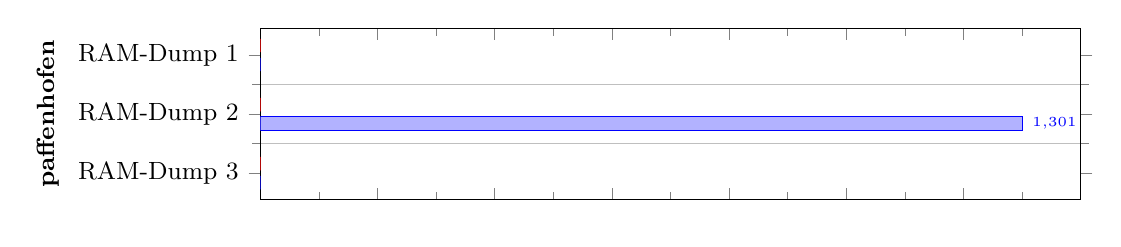
\begin{tikzpicture}
			\begin{axis}[
			xbar,
			width=12cm, 
			height=3cm, 
			ylabel style={align=center}, ylabel=\textbf{paffenhofen},
			y=0.75cm,
			symbolic y coords={RAM-Dump 3, RAM-Dump 2, RAM-Dump 1},
			label style={font=\small},
			tick label style={font=\small},
			ytick=data,
			xticklabels={,,},
            xmin = 0,
            xmax = 1400,
			nodes near coords, 
			nodes near coords align={horizontal},
			nodes near coords style={font=\tiny},
   			nodes near coords={\pgfmathfloatifflags{\pgfplotspointmeta}{0}{}{\pgfmathprintnumber{\pgfplotspointmeta}}},
			bar width=.17cm,
			enlarge y limits={abs=2*\pgfplotbarwidth},
			scaled x ticks=false,
			legend style={
				at={(0.5,-0.1)},
				anchor=north
			},
			legend columns=3,
    		yminorgrids = true,minor tick num=1
			]
				\addplot coordinates {
				(0,RAM-Dump 3) (1301,RAM-Dump 2) (0,RAM-Dump 1)
				};
				\addplot coordinates {
				(0,RAM-Dump 3) (0,RAM-Dump 2) (0,RAM-Dump 1)
				};
			\end{axis}
		\end{tikzpicture}
		\\[-7pt]
		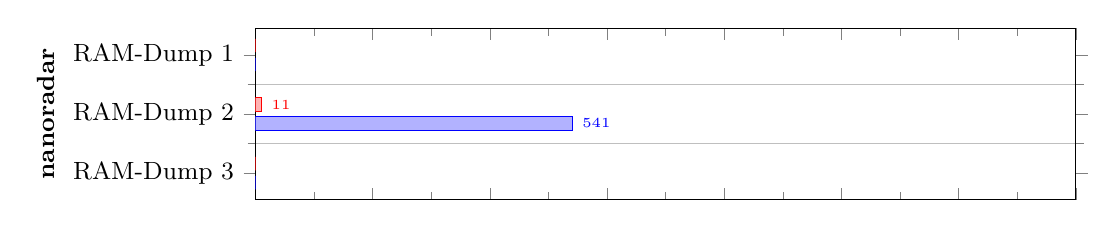
\begin{tikzpicture}
			\begin{axis}[
			xbar,
			width=12cm, 
			height=3cm, 
			ylabel style={align=center}, ylabel=\textbf{nanoradar},
			y=0.75cm,
			symbolic y coords={RAM-Dump 3, RAM-Dump 2, RAM-Dump 1},
			label style={font=\small},
			tick label style={font=\small},
			ytick=data,
			xticklabels={,,},
            xmin = 0,
            xmax = 1400,
			nodes near coords, 
			nodes near coords align={horizontal},
			nodes near coords style={font=\tiny},
   			nodes near coords={\pgfmathfloatifflags{\pgfplotspointmeta}{0}{}{\pgfmathprintnumber{\pgfplotspointmeta}}},
			bar width=.17cm,
			enlarge y limits={abs=2*\pgfplotbarwidth},
			scaled x ticks=false,
			legend style={
				at={(0.5,-0.1)},
				anchor=north
			},
			legend columns=3,
    		yminorgrids = true,minor tick num=1
			]
				\addplot coordinates {
				(0,RAM-Dump 3)  (541,RAM-Dump 2) (0,RAM-Dump 1)
				};
				\addplot coordinates {
				(0,RAM-Dump 3)  (11,RAM-Dump 2) (0,RAM-Dump 1)
				};
			\end{axis}
		\end{tikzpicture}
		\\[-7pt]
		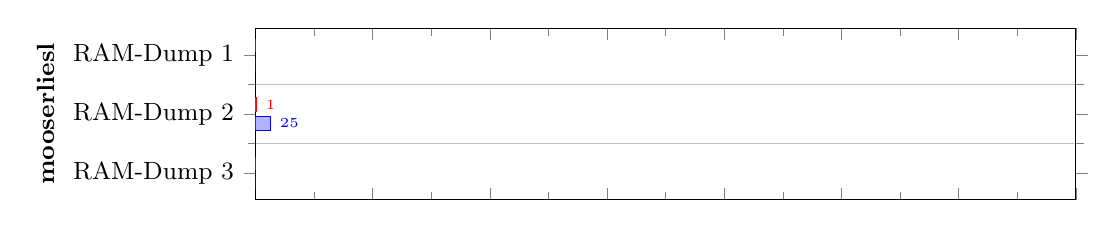
\begin{tikzpicture}
			\begin{axis}[
			xbar,
			width=12cm, 
			height=3cm, 
			ylabel style={align=center}, ylabel=\textbf{mooserliesl},
			y=0.75cm,
			symbolic y coords={RAM-Dump 3, RAM-Dump 2, RAM-Dump 1},
			label style={font=\small},
			tick label style={font=\small},
			ytick=data,
			xticklabels={,,},
            xmin = 0,
            xmax = 1400,
			nodes near coords, 
			nodes near coords align={horizontal},
			nodes near coords style={font=\tiny},
   			nodes near coords={\pgfmathfloatifflags{\pgfplotspointmeta}{0}{}{\pgfmathprintnumber{\pgfplotspointmeta}}},
			bar width=.17cm,
			enlarge y limits={abs=2*\pgfplotbarwidth},
			scaled x ticks=false,
			legend style={
				at={(0.5,-0.1)},
				anchor=north
			},
			legend columns=3,
    		yminorgrids = true,minor tick num=1
			]
				\addplot coordinates {
				(0,RAM-Dump 3)  (25,RAM-Dump 2) (0,RAM-Dump 1)
				};
				\addplot coordinates {
				(0,RAM-Dump 3)  (1,RAM-Dump 2) (0,RAM-Dump 1)
				};
			\end{axis}
		\end{tikzpicture}
		\\[-7pt]
		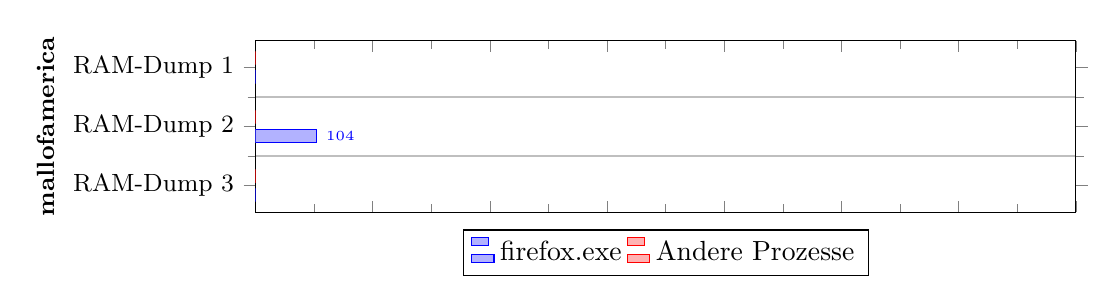
\begin{tikzpicture}
			\begin{axis}[
			xbar,
			width=12cm, 
			height=3cm, 
			ylabel style={align=center}, ylabel=\textbf{mallofamerica},
			y=0.75cm,
			symbolic y coords={RAM-Dump 3, RAM-Dump 2, RAM-Dump 1},
			label style={font=\small},
			tick label style={font=\small},
			ytick=data,
			xticklabels={,,},
            xmin = 0,
            xmax = 1400,
			nodes near coords, 
			nodes near coords align={horizontal},
			nodes near coords style={font=\tiny},
   			nodes near coords={\pgfmathfloatifflags{\pgfplotspointmeta}{0}{}{\pgfmathprintnumber{\pgfplotspointmeta}}},
			bar width=.17cm,
			enlarge y limits={abs=2*\pgfplotbarwidth},
			scaled x ticks=false,
			legend style={
				at={(0.5,-0.1)},
				anchor=north
			},
			legend columns=3,
    		yminorgrids = true,minor tick num=1
			]
				\addplot coordinates {
				(0,RAM-Dump 3)  (104,RAM-Dump 2) (0,RAM-Dump 1)
				};
				\addplot coordinates {
				(0,RAM-Dump 3)  (0,RAM-Dump 2) (0,RAM-Dump 1)
				};
				\legend{firefox.exe, Andere Prozesse}
			\end{axis}
		\end{tikzpicture}
	\end{tabular}
	}
	\caption{Gefundene Suchbegriffe im Firefox RAM}
	\label{chart:firefox-volatility-keywords}
\end{table}
				

%\begin{figure}[h!]
%	\centerline{\resizebox{\linewidth}{!}{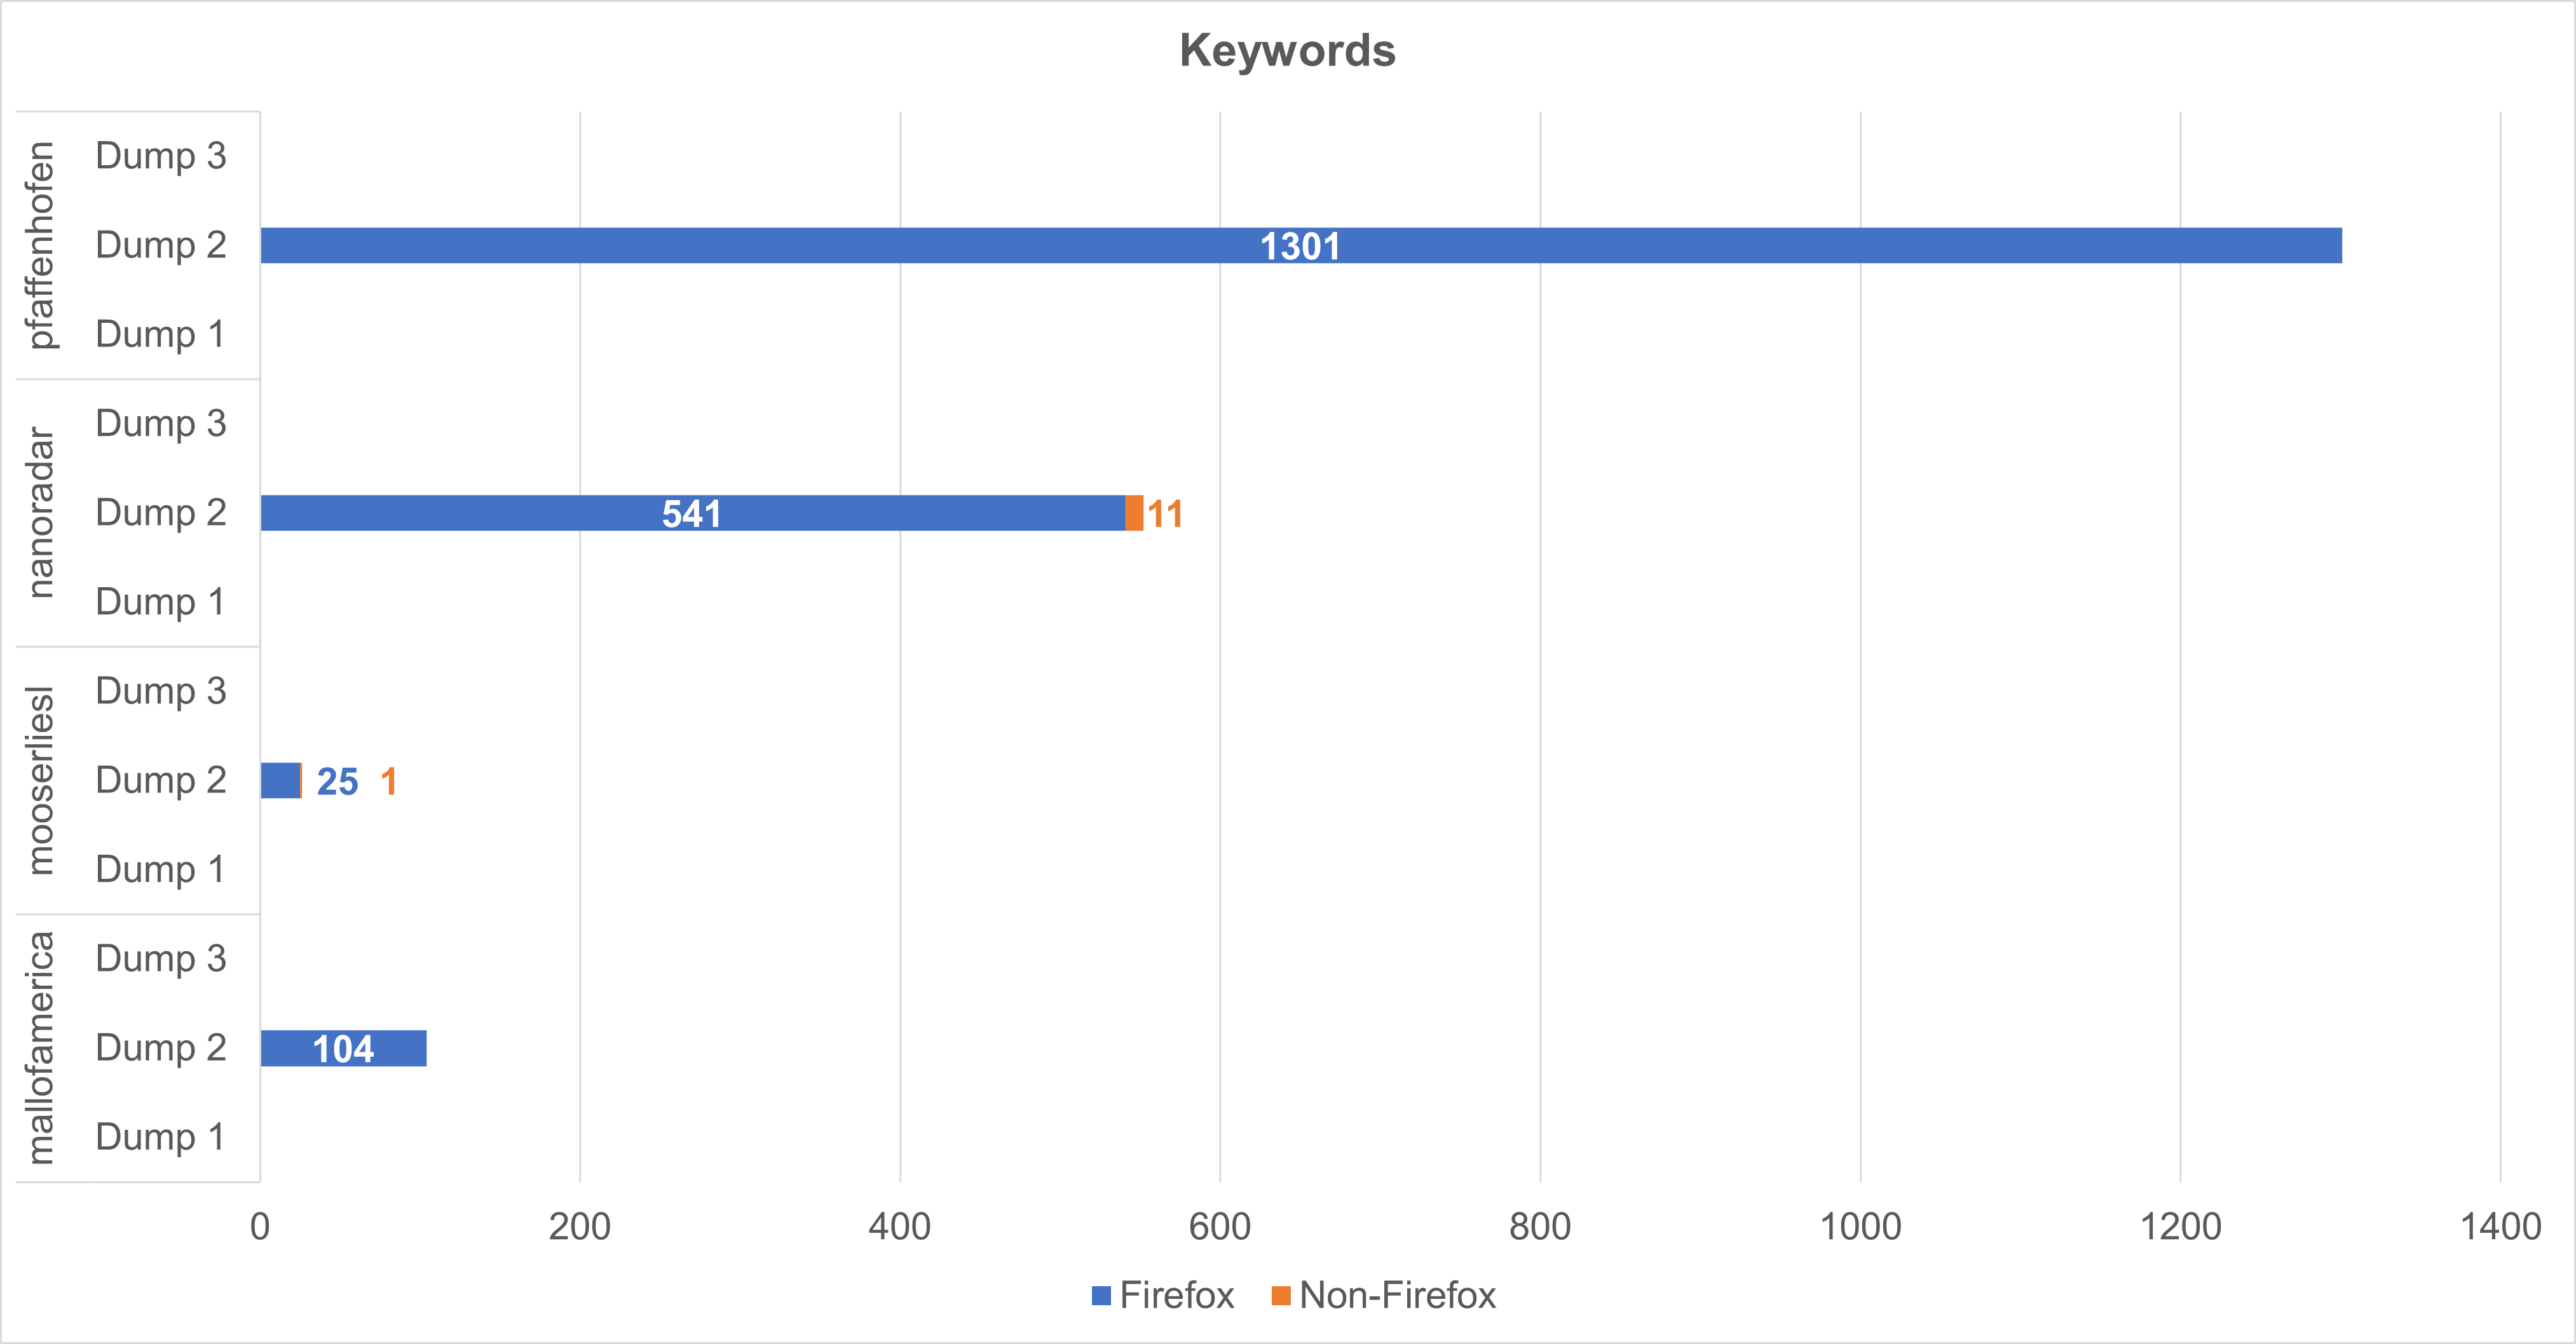
\includegraphics{bilder/volatility/firefox/keywords.png}}}
%	\label{chart:final-criteria}  
%	\caption{Keywords}
%\end{figure}

\paragraph*{Yara-Regel ``URLs``}

\begin{table}[h!]
	\resizebox{\linewidth}{!}{
	\begin{tabular}{l}	
		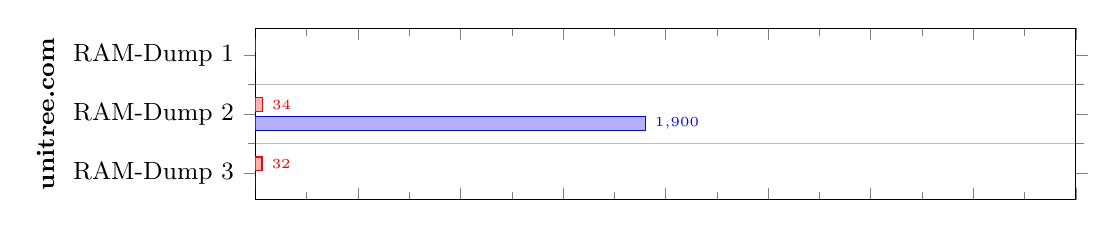
\begin{tikzpicture}
			\begin{axis}[
			xbar,
			width=12cm, 
			height=3cm, 
			ylabel style={align=center}, ylabel=\textbf{unitree.com},
			y=0.75cm,
			symbolic y coords={RAM-Dump 3, RAM-Dump 2, RAM-Dump 1},
			label style={font=\small},
			tick label style={font=\small},
			ytick=data,
			xticklabels={,,},
            xmin = 0,
            xmax = 4000,
			nodes near coords, 
			nodes near coords align={horizontal},
			nodes near coords style={font=\tiny},
   			nodes near coords={\pgfmathfloatifflags{\pgfplotspointmeta}{0}{}{\pgfmathprintnumber{\pgfplotspointmeta}}},
			bar width=.17cm,
			enlarge y limits={abs=2*\pgfplotbarwidth},
			scaled x ticks=false,
			legend style={
				at={(0.5,-0.1)},
				anchor=north
			},
			legend columns=3,
    		yminorgrids = true,minor tick num=1
			]
				\addplot coordinates {
				(0,RAM-Dump 3) (1900,RAM-Dump 2) (0,RAM-Dump 1)
				};
				\addplot coordinates {
				(32,RAM-Dump 3) (34,RAM-Dump 2) (0,RAM-Dump 1)
				};
			\end{axis}
		\end{tikzpicture}
		\\[-7pt]
		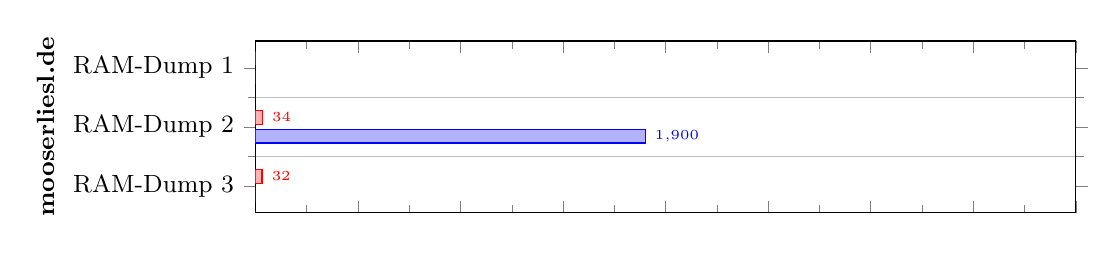
\begin{tikzpicture}
			\begin{axis}[
			xbar,
			width=12cm, 
			height=3cm, 
			ylabel style={align=center}, ylabel=\textbf{mooserliesl.de},
			y=0.75cm,
			symbolic y coords={RAM-Dump 3, RAM-Dump 2, RAM-Dump 1},
			label style={font=\small},
			tick label style={font=\small},
			ytick=data,
			xticklabels={,,},
            xmin = 0,
            xmax = 4000,
			nodes near coords, 
			nodes near coords align={horizontal},
			nodes near coords style={font=\tiny},
   			nodes near coords={\pgfmathfloatifflags{\pgfplotspointmeta}{0}{}{\pgfmathprintnumber{\pgfplotspointmeta}}},
			bar width=.17cm,
			enlarge y limits={abs=2*\pgfplotbarwidth},
			scaled x ticks=false,
			legend style={
				at={(0.5,-0.1)},
				anchor=north
			},
			legend columns=3,
    		yminorgrids = true,minor tick num=1
			]
				\addplot coordinates {
				(0,RAM-Dump 3) (1900,RAM-Dump 2) (0,RAM-Dump 1)
				};
				\addplot coordinates {
				(32,RAM-Dump 3) (34,RAM-Dump 2) (0,RAM-Dump 1)
				};
			\end{axis}
		\end{tikzpicture}	
		\\[-7pt]
		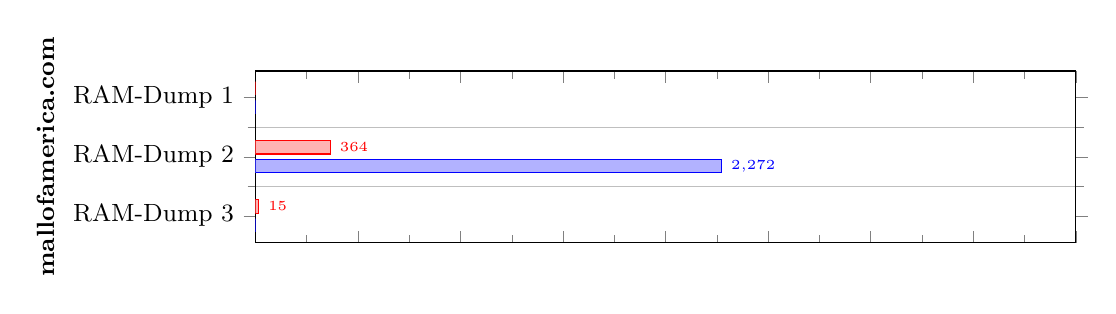
\begin{tikzpicture}
			\begin{axis}[
			xbar,
			width=12cm, 
			height=3cm, 
			ylabel style={align=center}, ylabel=\textbf{mallofamerica.com},
			y=0.75cm,
			symbolic y coords={RAM-Dump 3, RAM-Dump 2, RAM-Dump 1},
			label style={font=\small},
			tick label style={font=\small},
			ytick=data,
			xticklabels={,,},
            xmin = 0,
            xmax = 4000,
			nodes near coords, 
			nodes near coords align={horizontal},
			nodes near coords style={font=\tiny},
   			nodes near coords={\pgfmathfloatifflags{\pgfplotspointmeta}{0}{}{\pgfmathprintnumber{\pgfplotspointmeta}}},
			bar width=.17cm,
			enlarge y limits={abs=2*\pgfplotbarwidth},
			scaled x ticks=false,
			legend style={
				at={(0.5,-0.1)},
				anchor=north
			},
			legend columns=3,
    		yminorgrids = true,minor tick num=1
			]
				\addplot coordinates {
				(0,RAM-Dump 3) (2272,RAM-Dump 2) (0,RAM-Dump 1)
				};
				\addplot coordinates {
				(15,RAM-Dump 3) (364,RAM-Dump 2) (0,RAM-Dump 1)
				};
			\end{axis}
		\end{tikzpicture}
		\\[-7pt]
		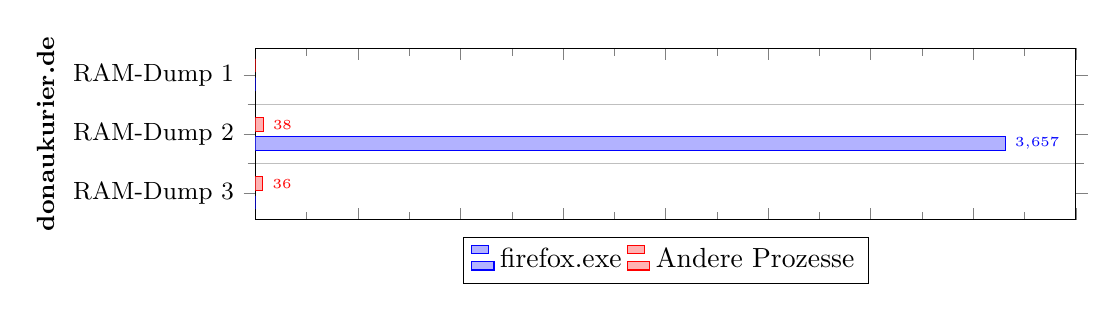
\begin{tikzpicture}
			\begin{axis}[
			xbar,
			width=12cm, 
			height=3cm, 
			ylabel style={align=center}, ylabel=\textbf{donaukurier.de},
			y=0.75cm,
			symbolic y coords={RAM-Dump 3, RAM-Dump 2, RAM-Dump 1},
			label style={font=\small},
			tick label style={font=\small},
			ytick=data,
			xticklabels={,,},
            xmin = 0,
            xmax = 4000,
			nodes near coords, 
			nodes near coords align={horizontal},
			nodes near coords style={font=\tiny},
   			nodes near coords={\pgfmathfloatifflags{\pgfplotspointmeta}{0}{}{\pgfmathprintnumber{\pgfplotspointmeta}}},
			bar width=.17cm,
			enlarge y limits={abs=2*\pgfplotbarwidth},
			scaled x ticks=false,
			legend style={
				at={(0.5,-0.1)},
				anchor=north
			},
			legend columns=3,
    		yminorgrids = true,minor tick num=1
			]
				\addplot coordinates {
				(0,RAM-Dump 3) (3657,RAM-Dump 2) (0,RAM-Dump 1)
				};
				\addplot coordinates {
				(36,RAM-Dump 3) (38,RAM-Dump 2) (0,RAM-Dump 1)
				};
				\legend{firefox.exe, Andere Prozesse}
			\end{axis}
		\end{tikzpicture}		
	\end{tabular}
	}
	\caption{Gefundene URLs im Firefox RAM}
	\label{chart:firefox-volatility-urls}
\end{table}

Es konnten in den Arbeitsspeicherabbildern alle besuchten URLs unitree.com, mooserliesl.de, mallofamerica.com sowie donaukurier.de identifiziert werden.
Wie in Tabelle \ref{chart:firefox-volatility-urls} gezeigt, wurden die meisten Artefakte nach dem Browsing Szenario mit geöffnetem Browser (RAM Dump 2) gefunden. Alle besuchten URLs wurden in diesem Dump sowohl in Firefox als auch anderen Prozessen gefunden, wobei die meisten Artefakte in Firefox Prozessen zu finden sind. Dabei wurde ``mooserliesl.de`` mit insgesamt 390 Artefakten am wenigsten gefunden, ``donaukurier.de`` mit über 3600 Artefakten am häufigsten.

Bemerkenswert ist, dass selbst URL Artefakte gefunden wurden nachdem der Browser geschlossen wurde (RAM Dump 3). Dabei wurde kein URL Artefakte in einem Firefox Prozess gefunden.
Anhand der PID $2252$ wurde festgestellt, dass sich alle URL Artefakte des dritten RAM Dumps in einem \textit{svchost.exe} Prozess mit der gleichen PID befinden. Unter dem \textit{Service Host} Prozess laufen gruppierte Windows-Dienste, um Ressourcen zu sparen und die Systemleistung zu verbessern.
Volatility bietet das Plugin \textit{svcscan} an, mit dem alle laufenden Dienste ausgegeben werden können.
Bei Anwendung auf den dritten RAM Dump wurde jedoch zu keinem Dienst eine PID angegeben, wordurch der Dienst mit den URL Artefakten nicht im RAM identifiziert werden konnte. \cite{Nicholasswhite.05.06.2023}
Stattdessen wurde der dritte Snapshot aufgetaut, um im laufenden Windowsbetrieb den Dienst mithilfe des Process Explorers zu identifizieren.
Wie in Abbildung \ref{chart:svchost-dnscache} gezeigt, wurde anhand der PID $2252$ der Dienst \textit{DNSCache} ermittelt.
\begin{figure}[h!]
	\centerline{\resizebox{\linewidth}{!}{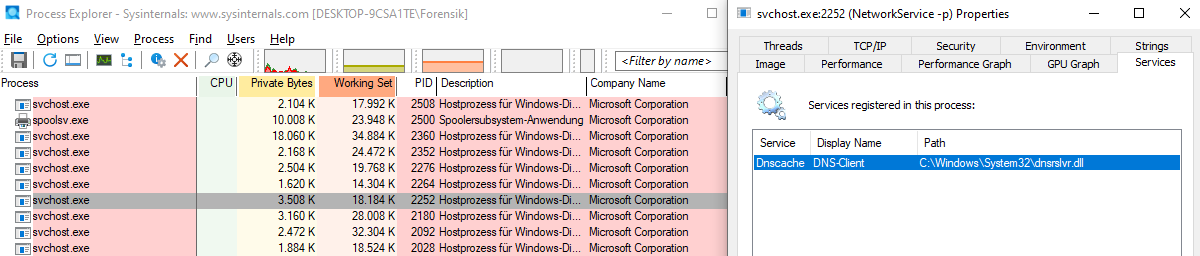
\includegraphics{bilder/firefox-dnscache.png}}}
	\caption{Unter dem SVChost-Prozess PID $2252$ läuft der DNSCache-Dienst.}
	\label{chart:svchost-dnscache}  
\end{figure}
Der DNSCache-Dienst unter Windows ist ein Teil des Betriebssystems, der für die Übersetzung von Domainnamen in IP-Adressen verantwortlich ist. Der DNSCache-Dienst speichert DNS-Anfragen und Antworten temporär, umd wiederholte DNS-Anfragen zu beschleunigen. \cite{MicrosoftLearn.05.06.2023}
Nach Löschen des DNSCaches mit dem Kommandozeilenbefehl \texttt{ipconfig /flushdns}, dem Schließen aller Process Monitor Instanzen sowie Beenden des DNSCaches Services wurde erneut ein RAM-Dump durchgeführt. Dort wurden keine URL Artefakte mehr gefunden.

\paragraph*{Yara-Regel ``E-Mail``}

\begin{table}[h!]
	\resizebox{\linewidth}{!}{
	\begin{tabular}{r}	
		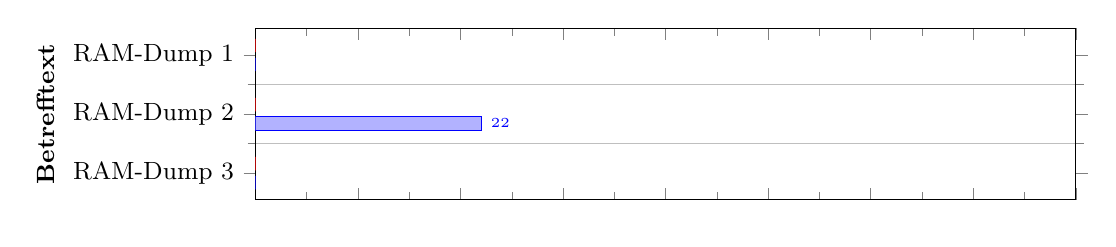
\begin{tikzpicture}
			\begin{axis}[
			xbar,
			width=12cm, 
			height=3cm, 
			ylabel style={align=center}, ylabel=\textbf{Betrefftext},
			y=0.75cm,
			symbolic y coords={RAM-Dump 3, RAM-Dump 2, RAM-Dump 1},
			label style={font=\small},
			tick label style={font=\small},
			ytick=data,
			xticklabels={,,},
            xmin = 0,
            xmax = 80,
			nodes near coords, 
			nodes near coords align={horizontal},
			nodes near coords style={font=\tiny},
   			nodes near coords={\pgfmathfloatifflags{\pgfplotspointmeta}{0}{}{\pgfmathprintnumber{\pgfplotspointmeta}}},
			bar width=.17cm,
			enlarge y limits={abs=2*\pgfplotbarwidth},
			scaled x ticks=false,
			legend style={
				at={(0.5,-0.1)},
				anchor=north
			},
			legend columns=3,
    		yminorgrids = true,minor tick num=1
			]
				\addplot coordinates {
				(0,RAM-Dump 3) (22,RAM-Dump 2) (0,RAM-Dump 1)
				};
				\addplot coordinates {
				(0,RAM-Dump 3) (0,RAM-Dump 2) (0,RAM-Dump 1)
				};
%				\legend{firefox.exe, Andere Prozesse}
			\end{axis}
		\end{tikzpicture}
		\\[-7pt]
		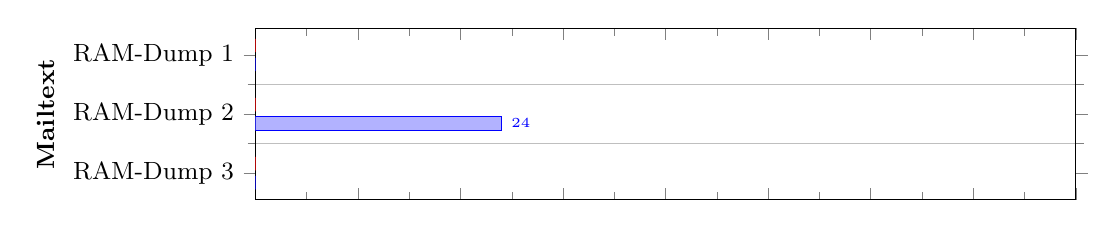
\begin{tikzpicture}
			\begin{axis}[
			xbar,
			width=12cm, 
			height=3cm, 
			ylabel style={align=center}, ylabel=\textbf{Mailtext},
			y=0.75cm,
			symbolic y coords={RAM-Dump 3, RAM-Dump 2, RAM-Dump 1},
			label style={font=\small},
			tick label style={font=\small},
			ytick=data,
			xticklabels={,,},
            xmin = 0,
            xmax = 80,
			nodes near coords, 
			nodes near coords align={horizontal},
			nodes near coords style={font=\tiny},
   			nodes near coords={\pgfmathfloatifflags{\pgfplotspointmeta}{0}{}{\pgfmathprintnumber{\pgfplotspointmeta}}},
			bar width=.17cm,
			enlarge y limits={abs=2*\pgfplotbarwidth},
			scaled x ticks=false,
			legend style={
				at={(0.5,-0.1)},
				anchor=north
			},
			legend columns=3,
    		yminorgrids = true,minor tick num=1
			]
				\addplot coordinates {
				(0,RAM-Dump 3) (24,RAM-Dump 2) (0,RAM-Dump 1)
				};
				\addplot coordinates {
				(0,RAM-Dump 3) (0,RAM-Dump 2) (0,RAM-Dump 1)
				};
%				\legend{firefox.exe, Andere Prozesse}
			\end{axis}
		\end{tikzpicture}	
		\\[-7pt]
		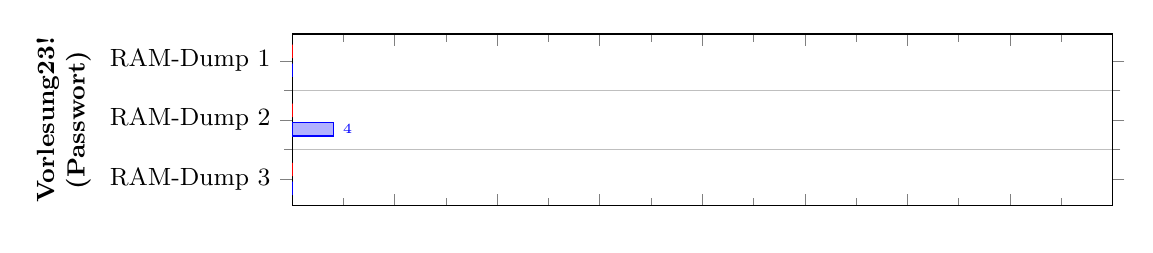
\begin{tikzpicture}
			\begin{axis}[
			xbar,
			width=12cm, 
			height=3cm, 
			ylabel style={align=center}, ylabel=\textbf{Vorlesung23!}\\\textbf{(Passwort)},
			y=0.75cm,
			symbolic y coords={RAM-Dump 3, RAM-Dump 2, RAM-Dump 1},
			label style={font=\small},
			tick label style={font=\small},
			ytick=data,
			xticklabels={,,},
            xmin = 0,
            xmax = 80,
			nodes near coords, 
			nodes near coords align={horizontal},
			nodes near coords style={font=\tiny},
   			nodes near coords={\pgfmathfloatifflags{\pgfplotspointmeta}{0}{}{\pgfmathprintnumber{\pgfplotspointmeta}}},
			bar width=.17cm,
			enlarge y limits={abs=2*\pgfplotbarwidth},
			scaled x ticks=false,
			legend style={
				at={(0.5,-0.1)},
				anchor=north
			},
			legend columns=3,
    		yminorgrids = true,minor tick num=1
			]
				\addplot coordinates {
				(0,RAM-Dump 3) (4,RAM-Dump 2) (0,RAM-Dump 1)
				};
				\addplot coordinates {
				(0,RAM-Dump 3) (0,RAM-Dump 2) (0,RAM-Dump 1)
				};
%				\legend{firefox.exe, Andere Prozesse}
			\end{axis}
		\end{tikzpicture}
		\\[-7pt]
		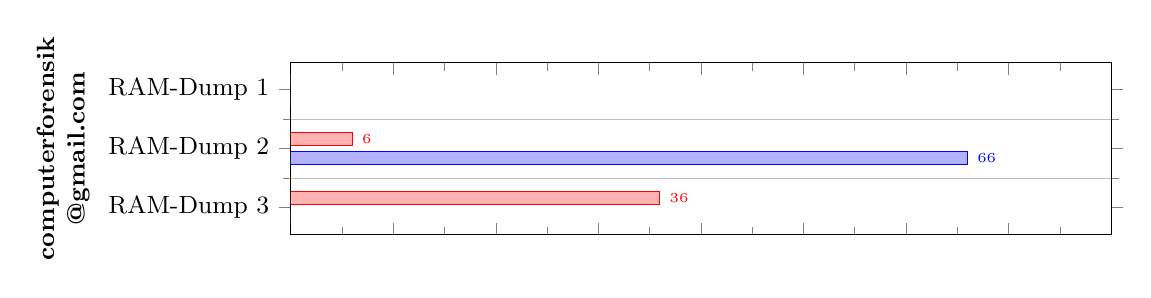
\begin{tikzpicture}
			\begin{axis}[
			xbar,
			width=12cm, 
			height=3cm, 
			ylabel style={align=center}, ylabel=\textbf{computerforensik}\\\textbf{@gmail.com},
			y=0.75cm,
			symbolic y coords={RAM-Dump 3, RAM-Dump 2, RAM-Dump 1},
			label style={font=\small},
			tick label style={font=\small},
			ytick=data,
			xticklabels={,,},
            xmin = 0,
            xmax = 80,
			nodes near coords, 
			nodes near coords align={horizontal},
			nodes near coords style={font=\tiny},
   			nodes near coords={\pgfmathfloatifflags{\pgfplotspointmeta}{0}{}{\pgfmathprintnumber{\pgfplotspointmeta}}},
			bar width=.17cm,
			enlarge y limits={abs=2*\pgfplotbarwidth},
			scaled x ticks=false,
			legend style={
				at={(0.5,-0.1)},
				anchor=north
			},
			legend columns=3,
    		yminorgrids = true,minor tick num=1
			]
				\addplot coordinates {
				(0,RAM-Dump 3) (66,RAM-Dump 2) (0,RAM-Dump 1)
				};
				\addplot coordinates {
				(36,RAM-Dump 3) (6,RAM-Dump 2) (0,RAM-Dump 1)
				};
%				\legend{firefox.exe, Andere Prozesse}
			\end{axis}
		\end{tikzpicture}	
		\\[-7pt]
		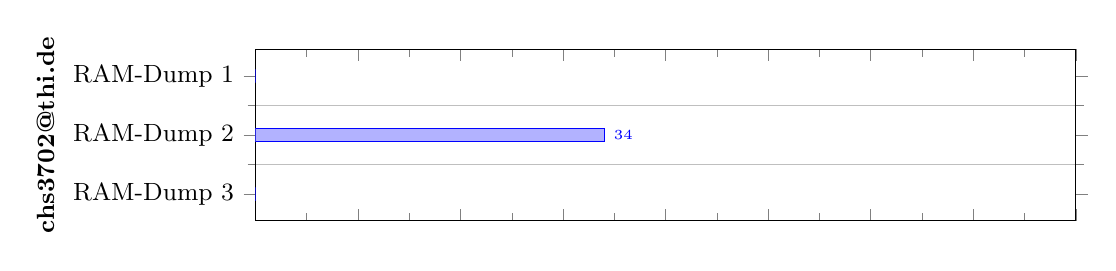
\begin{tikzpicture}
			\begin{axis}[
			xbar,
			width=12cm, 
			height=3cm, 
			ylabel style={align=center}, ylabel=\textbf{chs3702@thi.de},
			y=0.75cm,
			symbolic y coords={RAM-Dump 3, RAM-Dump 2, RAM-Dump 1},
			label style={font=\small},
			tick label style={font=\small},
			ytick=data,
			xticklabels={,,},
            xmin = 0,
            xmax = 80,
			nodes near coords, 
			nodes near coords align={horizontal},
			nodes near coords style={font=\tiny},
   			nodes near coords={\pgfmathfloatifflags{\pgfplotspointmeta}{0}{}{\pgfmathprintnumber{\pgfplotspointmeta}}},
			bar width=.17cm,
			enlarge y limits={abs=2*\pgfplotbarwidth},
			scaled x ticks=false,
			legend style={
				at={(0.5,-0.1)},
				anchor=north
			},
			legend columns=3,
    		yminorgrids = true,minor tick num=1
			]
				\addplot coordinates {
				(0,RAM-Dump 3) (34,RAM-Dump 2) (0,RAM-Dump 1)
				};
%				\legend{firefox.exe, Andere Prozesse}
			\end{axis}
		\end{tikzpicture}
		\\[-7pt]
		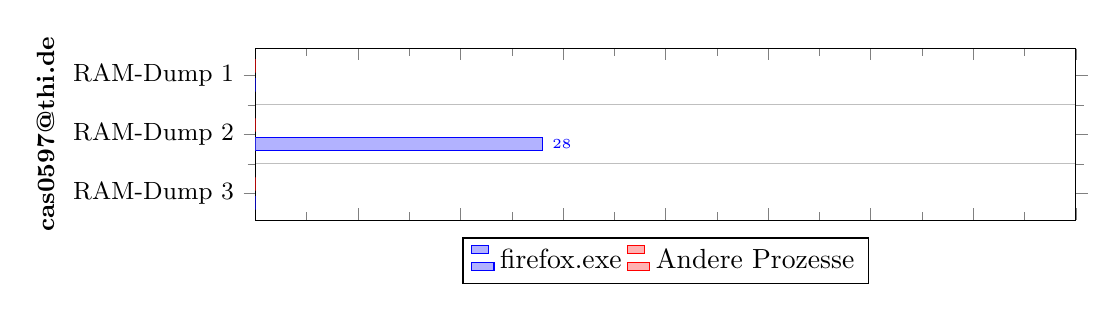
\begin{tikzpicture}
			\begin{axis}[
			xbar,
			width=12cm, 
			height=3cm, 
			ylabel style={align=center}, ylabel=\textbf{cas0597@thi.de},
			y=0.75cm,
			symbolic y coords={RAM-Dump 3, RAM-Dump 2, RAM-Dump 1},
			label style={font=\small},
			tick label style={font=\small},
			ytick=data,
			xticklabels={,,},
            xmin = 0,
            xmax = 80,
			nodes near coords, 
			nodes near coords align={horizontal},
			nodes near coords style={font=\tiny},
   			nodes near coords={\pgfmathfloatifflags{\pgfplotspointmeta}{0}{}{\pgfmathprintnumber{\pgfplotspointmeta}}},
			bar width=.17cm,
			enlarge y limits={abs=2*\pgfplotbarwidth},
			scaled x ticks=false,
			legend style={
				at={(0.5,-0.1)},
				anchor=north
			},
			legend columns=3,
    		yminorgrids = true,minor tick num=1
			]
				\addplot coordinates {
				(0,RAM-Dump 3) (28,RAM-Dump 2) (0,RAM-Dump 1)
				};
				\addplot coordinates {
				(0,RAM-Dump 3) (0,RAM-Dump 2) (0,RAM-Dump 1)
				};
				\legend{firefox.exe, Andere Prozesse}
			\end{axis}
		\end{tikzpicture}
				%	\begin{axis}[]
		%	\legend{Logfile 1, Logfile 2}
		%	\end{axis}

	\end{tabular}
	}
	\caption{Gefundene E-Mail Artefakte im Firefox RAM}
	\label{chart:firefox-volatility-mail}
\end{table}

%\begin{figure}[h!]
%	\centerline{\resizebox{\linewidth}{!}{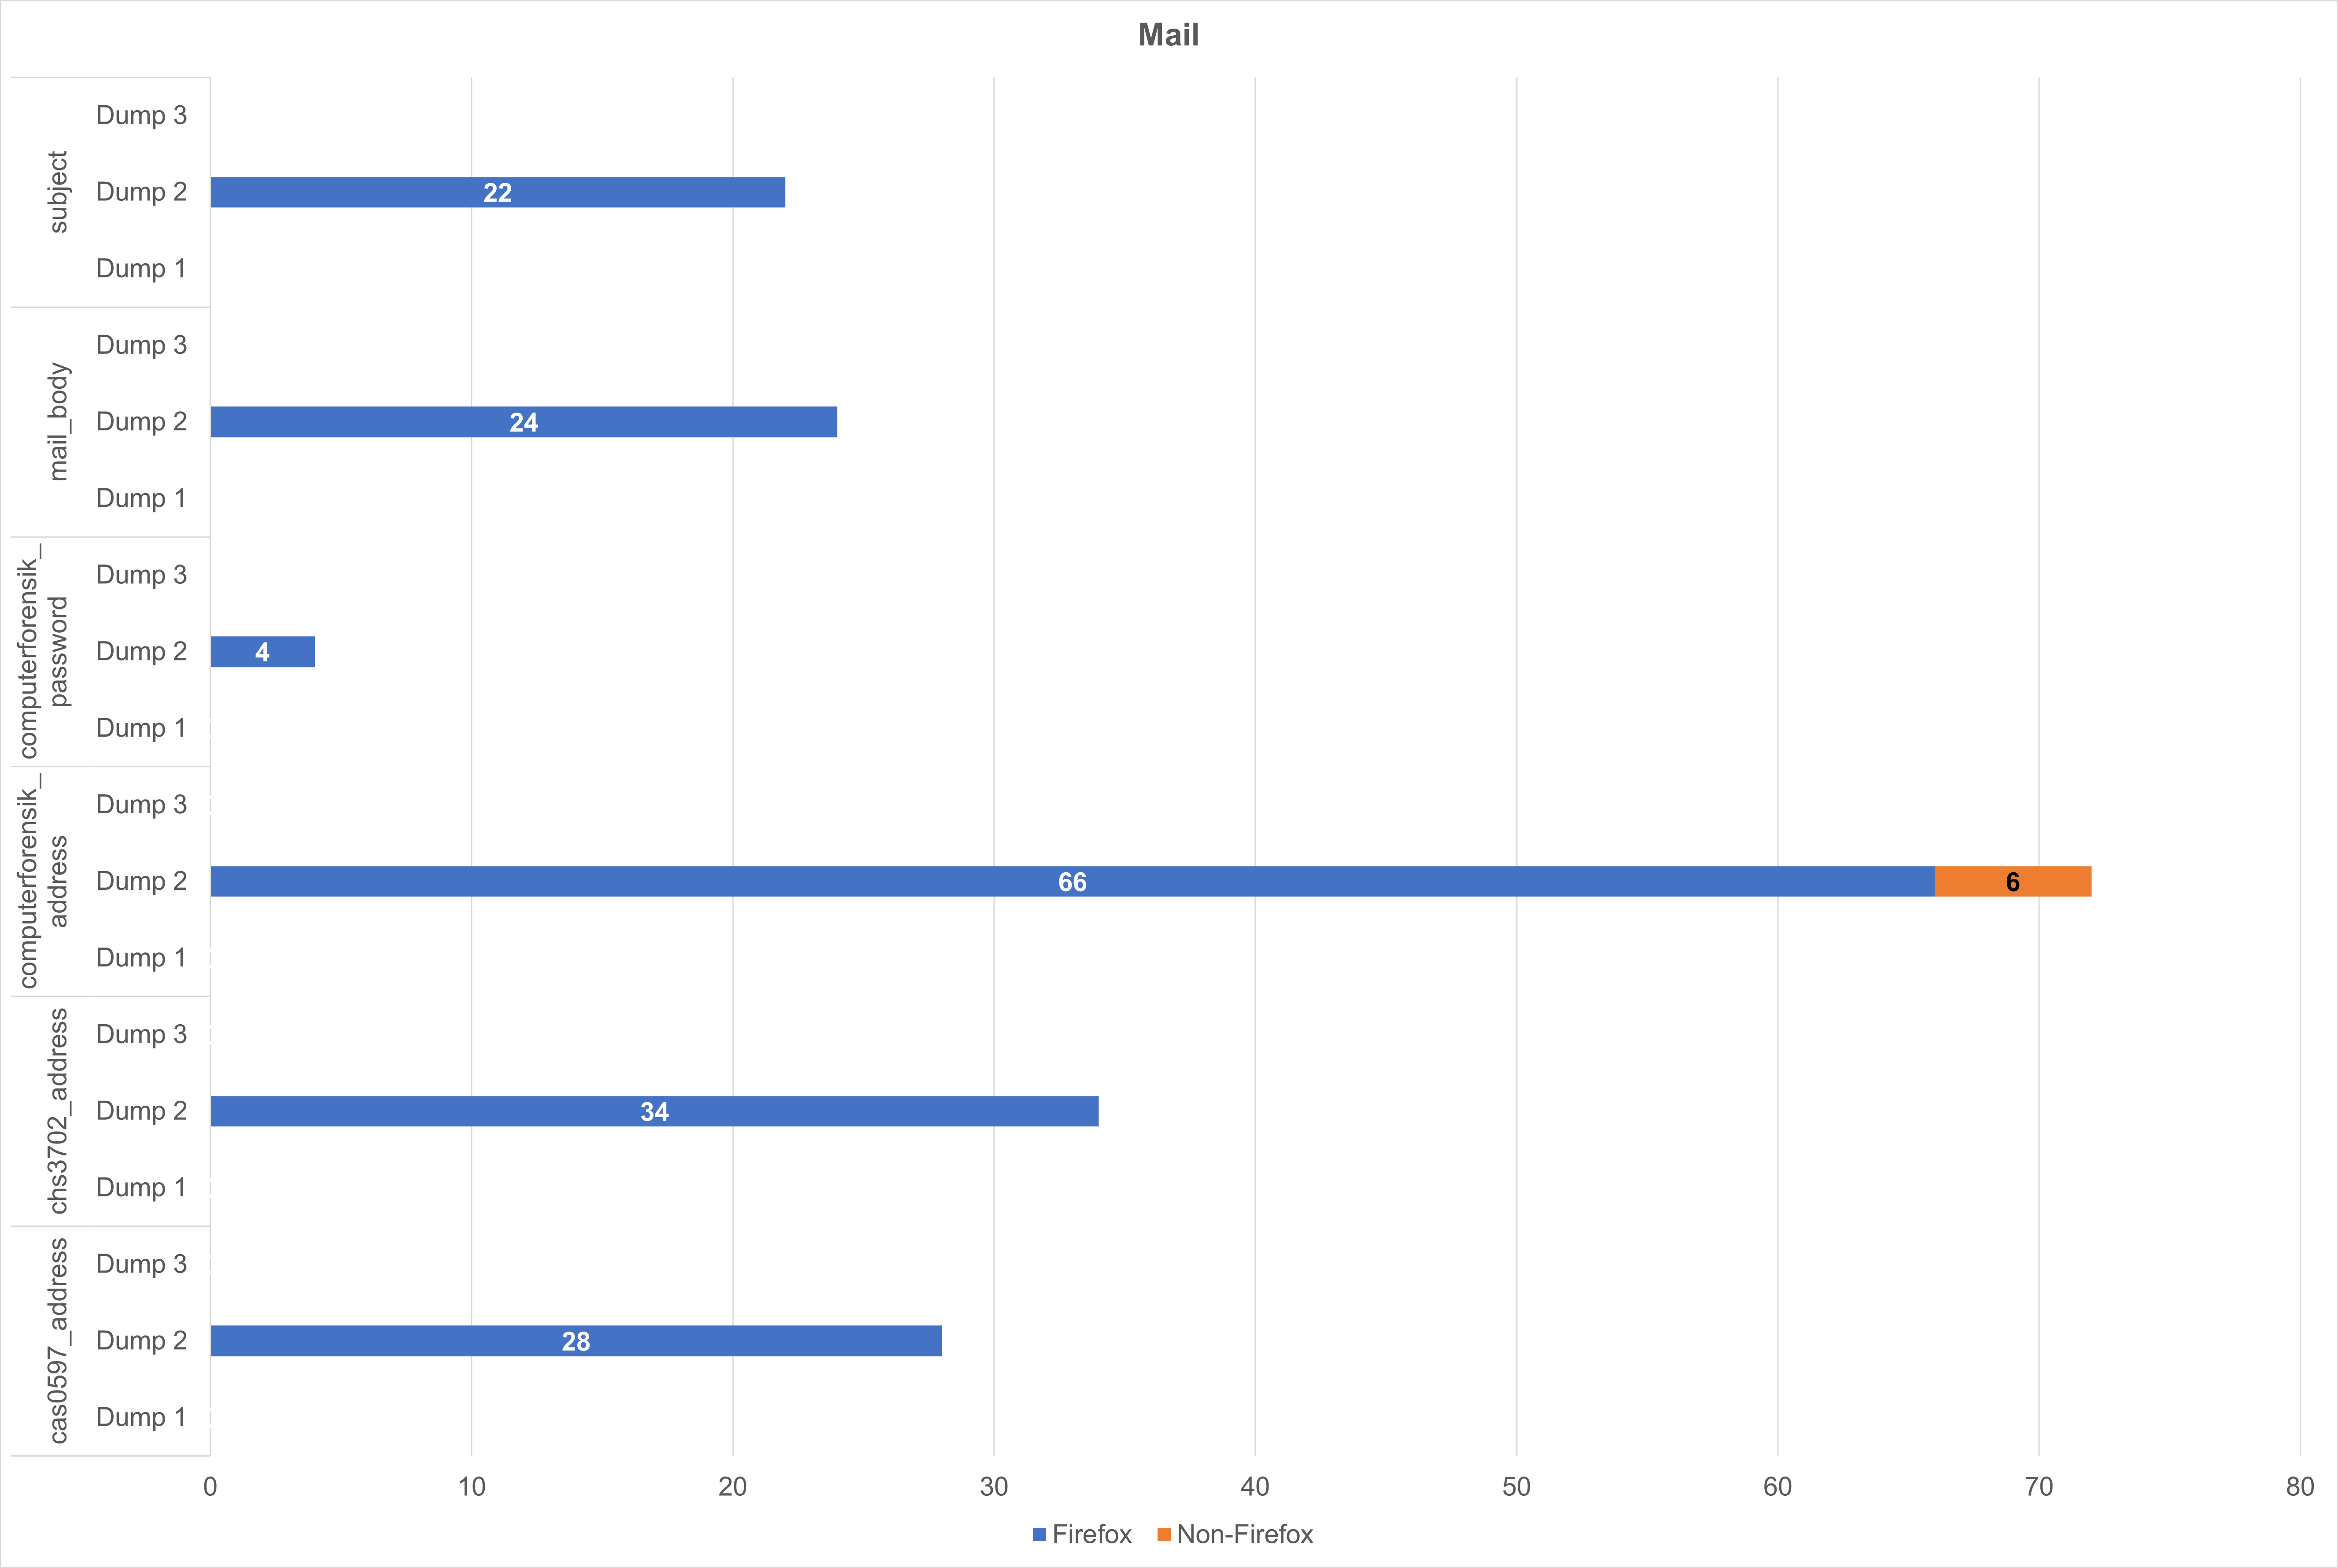
\includegraphics{bilder/volatility/firefox/mail.png}}}
%	\label{chart:final-criteria}  
%	\caption{Mail}
%\end{figure}
Es konnten alle E-Mail Artefakte des Browsing Szenarios gefunden werden.
Wie in Abbildung \ref{chart:firefox-volatility-mail} gezeigt, befindensich die Artefakte ausschließlich im zweiten Firefox RAM Dump, nach dem Browsing Szenario mit geöffnetem Browser.
Unter den gefundenen Artefakten befindet sich mit zwölf Vorkommen am häufigsten die Absenderadresse ``computerforensikvl@gmail.com``. Dieses Artefakt wurde als einziges Mail-Artefakt in anderen Prozesses außer Firefox gefunden.

Bemerkenswert ist, dass das Passwort des Google-Accounts, mit dem die E-Mails verschickt wurden, vier mal als Klartext im RAM gefunden wurden. Das Passwort wurde in je zwei Firefox Prozessen mit den PIDs 7420 und 8424 zwei mal gefunden. Tabelle \ref{tab:firefox-mapping-virtaddr-to-byteoffset} zeigt die virtuellen Speicheradressen der Artefakte aus der Yarascan Ausgabe.
\begin{table}[h!]
\resizebox{\linewidth}{!}{
\begin{tabular}{|c|c|c|ll}
\cline{1-3}
\textbf{Virtuelle Speicheradresse} & \textbf{PID} & \textbf{Byte-Offset in extrahierter Speicherseite} &  &  \\ \cline{1-3}
0xb9ce29180c8                      & 7420         & 0x11dd40c8                                         &  &  \\ \cline{1-3}
0x2859f4ffd4e0                     & 7420         & 0x12e234e0                                         &  &  \\ \cline{1-3}
0x24083b41858                      & 8424         & 0x583858                                           &  &  \\ \cline{1-3}
0x240840e5b08                      & 8424         & 0x96bb08                                           &  &  \\ \cline{1-3}
\end{tabular}
}
\caption{Abbildung der virtellen Speicheradressen im Firefox-RAM der gefundenen Strings auf Byte-Offsets der entsprechenden Speicherseiten}
\label{tab:firefox-mapping-virtaddr-to-byteoffset}
\end{table}

Zu diesen Artefakten wurde gemäß Methodik in Kapitel \ref{subsubsection:ergebnisse-firefox-uncommonlocations-analysemitvolatility} der String Kontext -- also die Zeichen vor und nach dem gefundenen Artefakt im Speicherbereich -- ermittelt. Dazu wurde mithilfe des Volatility memmap-Plugins die Abbildung der virtuellen Speicheradressen auf den Byte-Offset in der extrahierten Speicherseite des Prozesses ermittelt. 

\begin{figure}[h!]
	\centering
	\subcaptionbox{Byte-Offset 0x11dd40c8}{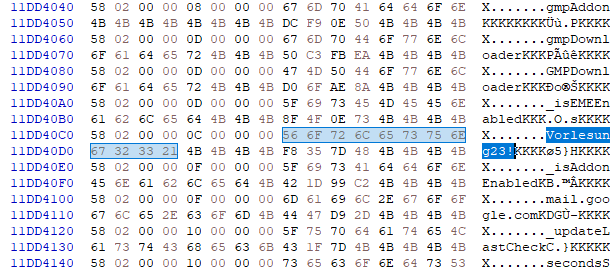
\includegraphics[width=0.47\textwidth]{bilder/volatility/firefox/password_0xb9ce29180c8_7420.png}}%
	\hfill
	\subcaptionbox{Byte-Offset 0x12e234e0}{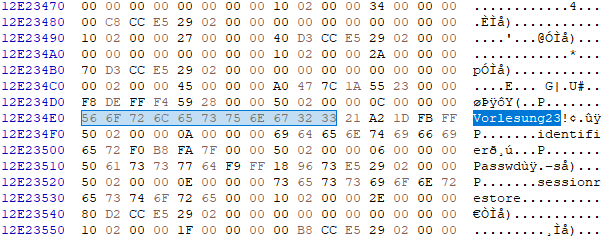
\includegraphics[width=0.47\textwidth]{bilder/volatility/firefox/password_0x2859f4ffd4e0_7420.png}}%
	\caption{Passwort-Klartext in Firefox Speicherseiten von PID 7420}
	\label{img:firefox-pw-offset-pid-7420}  
\end{figure}
Wie in Abbildung \ref{img:firefox-pw-offset-pid-7420} gezeigt, sind in der Speicherseite des Prozesses mit PID $7420$ konnte vor und nach dem gefundenen Passwort am Byte-Offset $0xb9ce29180c8$ neben der Gmail-URL ``mail.google.com`` Code-Fragmente der \textit{Gecko-Engine} zu finden. Dieser Teil des Firefox Browsers ist für das Rendering von Webinhalten verantwortlich, einschließlich HTML, CSS, JavaScript und anderen Medienformaten wie Bildern, Audio und Video. \cite{MozillaWiki.05.06.2023}
In der gleichen Datei konnte nach dem gefundenen Passwort am Byte-Offset $0x12e234e0$ die Strings ``Passwd`` sowie ``sessionrestore`` (siehe Common Location \textit{Sessionstore} in Anhang \ref{subsubsection:appendix-firefox-common-locations-writefile-operations}) identifiziert werden. 

\begin{figure}[h!]
	\centering
	\subcaptionbox{Byte-Offset 0x583858}{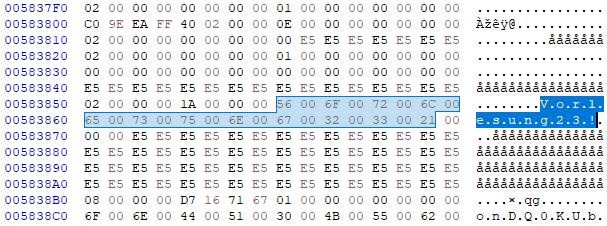
\includegraphics[width=0.47\textwidth]{bilder/volatility/firefox/password_0x24083b41858_8424.png}}%
	\hfill
	\subcaptionbox{Byte-Offset 0x96bb08}{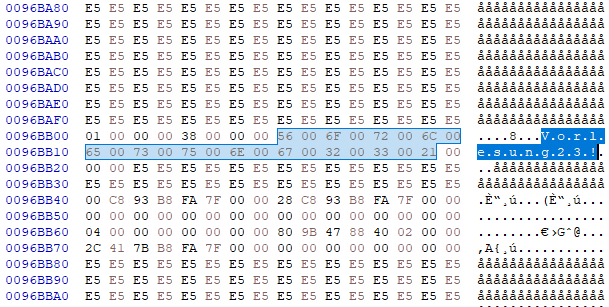
\includegraphics[width=0.47\textwidth]{bilder/volatility/firefox/password_0x240840e5b08_8424.png}}%
	\caption{Passwort-Klartext in Firefox Speicherseiten von PID 8424}
	\label{img:firefox-pw-offset-pid-8424}  
\end{figure}
Wie in Abbildung \ref{img:firefox-pw-offset-pid-8424} gezeigt, können in den Byte-Offsets der gefundenen Passwörter in der Speicherseite der PID 8424 konnten kein Kontext ermittelt werden. Im Gegensatz zur Speicherseite der PID 7420 wird das Passwort dort mit 2 Bytes pro Zeichen enkodiert. Das eine Unicode-Zeichenenkodierung vermuten.

\paragraph*{Yara-Regel ``DK-Logo``}
Wie in Abbildung \ref{chart:firefox-volatility-image} gezeigt, wurde das im Browsing Szenario geöffnete Donaukurier Logo ausschließlich im zweiten RAM Dump in drei mal in Firefox Prozessen gefunden.
\begin{table}[h!]
	\resizebox{\linewidth}{!}{
	\begin{tabular}{r}
		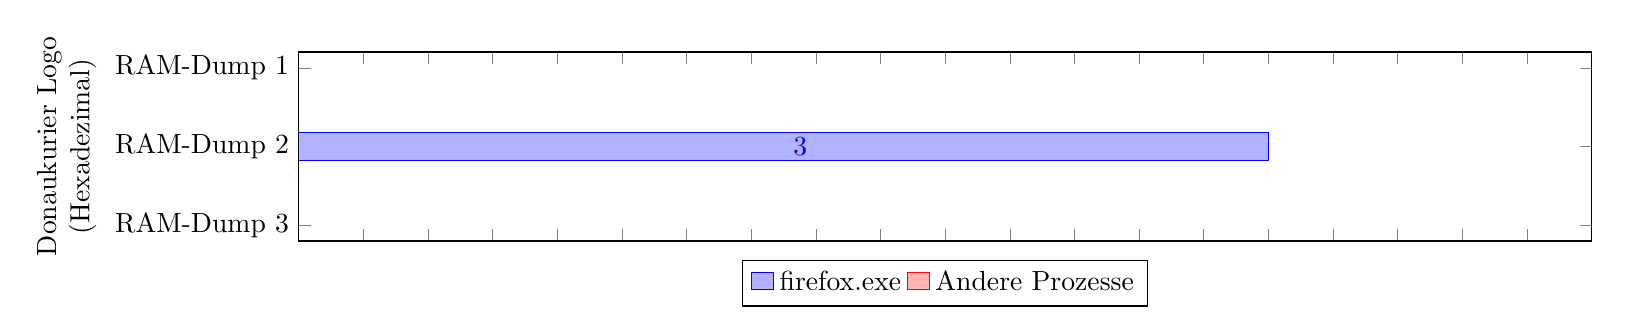
\begin{tikzpicture}
			\begin{axis}[
			xbar stacked,
			width=18cm, 
			height=12cm, 
			ylabel style={align=center}, ylabel=Donaukurier Logo\\(Hexadezimal),
			y=1cm,
			symbolic y coords={RAM-Dump 3, RAM-Dump 2, RAM-Dump 1},
			ytick=data,
			xticklabels={,,},
            xmin = 0,
            xmax = 4,
			nodes near coords, 
			nodes near coords align={horizontal},
			legend style={
				at={(0.5,-0.1)},
				anchor=north
			},
			legend columns=2
			]
				\addplot coordinates {
				(0,RAM-Dump 3) (3,RAM-Dump 2) (0,RAM-Dump 1)
				};
				\addplot coordinates {
				(0,RAM-Dump 3) (0,RAM-Dump 2) (0,RAM-Dump 1)
				};
				\legend{firefox.exe, Andere Prozesse}
			\end{axis}
		\end{tikzpicture}
	\end{tabular}
	}
	\caption{Gefundener Hexadezimalwert des Donaukurier-Logos im Firefox RAM}
	\label{chart:firefox-volatility-image}
\end{table}
%\begin{figure}[h!]
%	\centerline{\resizebox{\linewidth}{!}{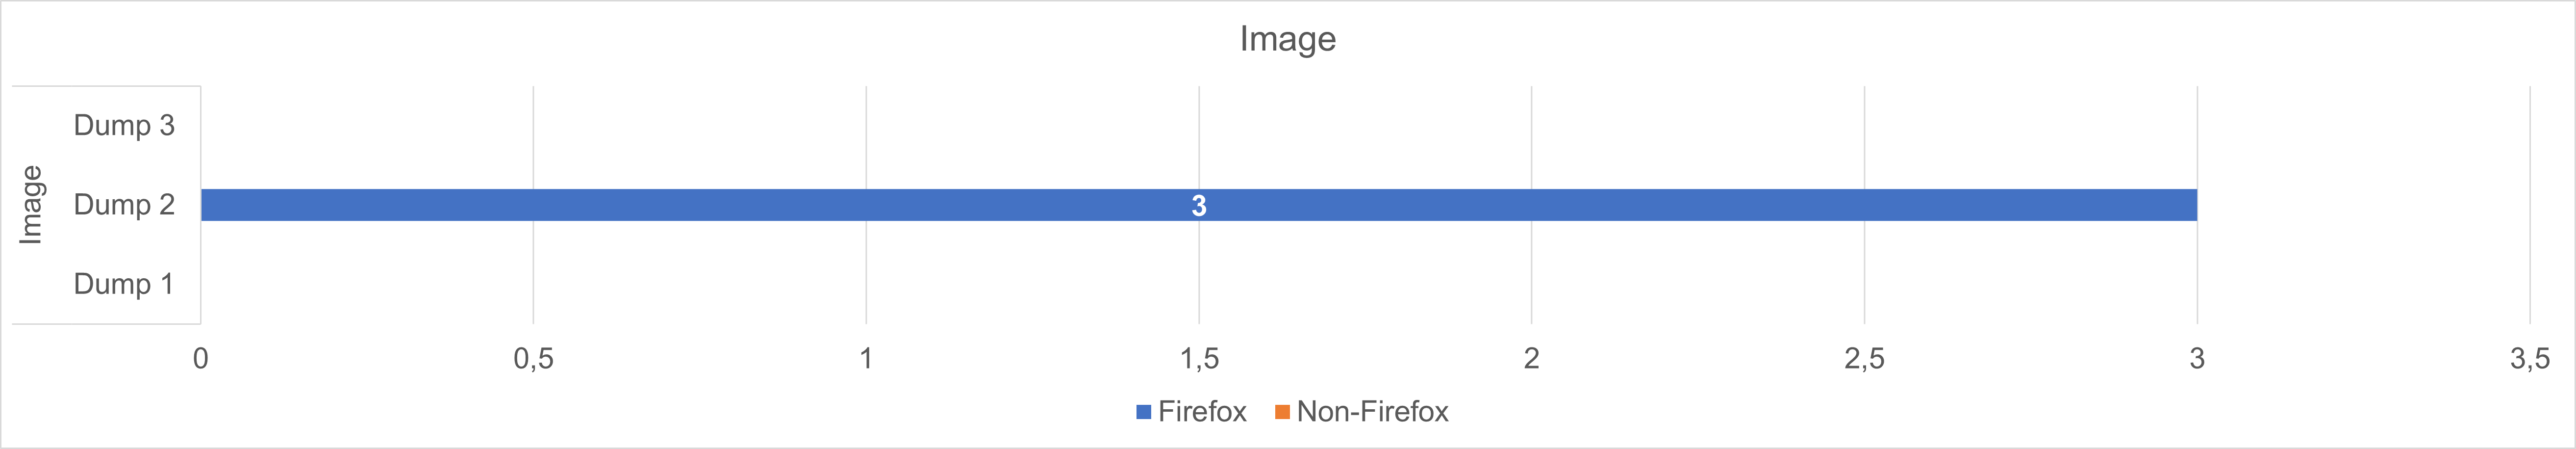
\includegraphics{bilder/volatility/firefox/image.png}}}
%	\label{chart:final-criteria}  
%	\caption{Image}
%\end{figure}



%\begin{figure}[h!]
%	\centerline{\resizebox{\linewidth}{!}{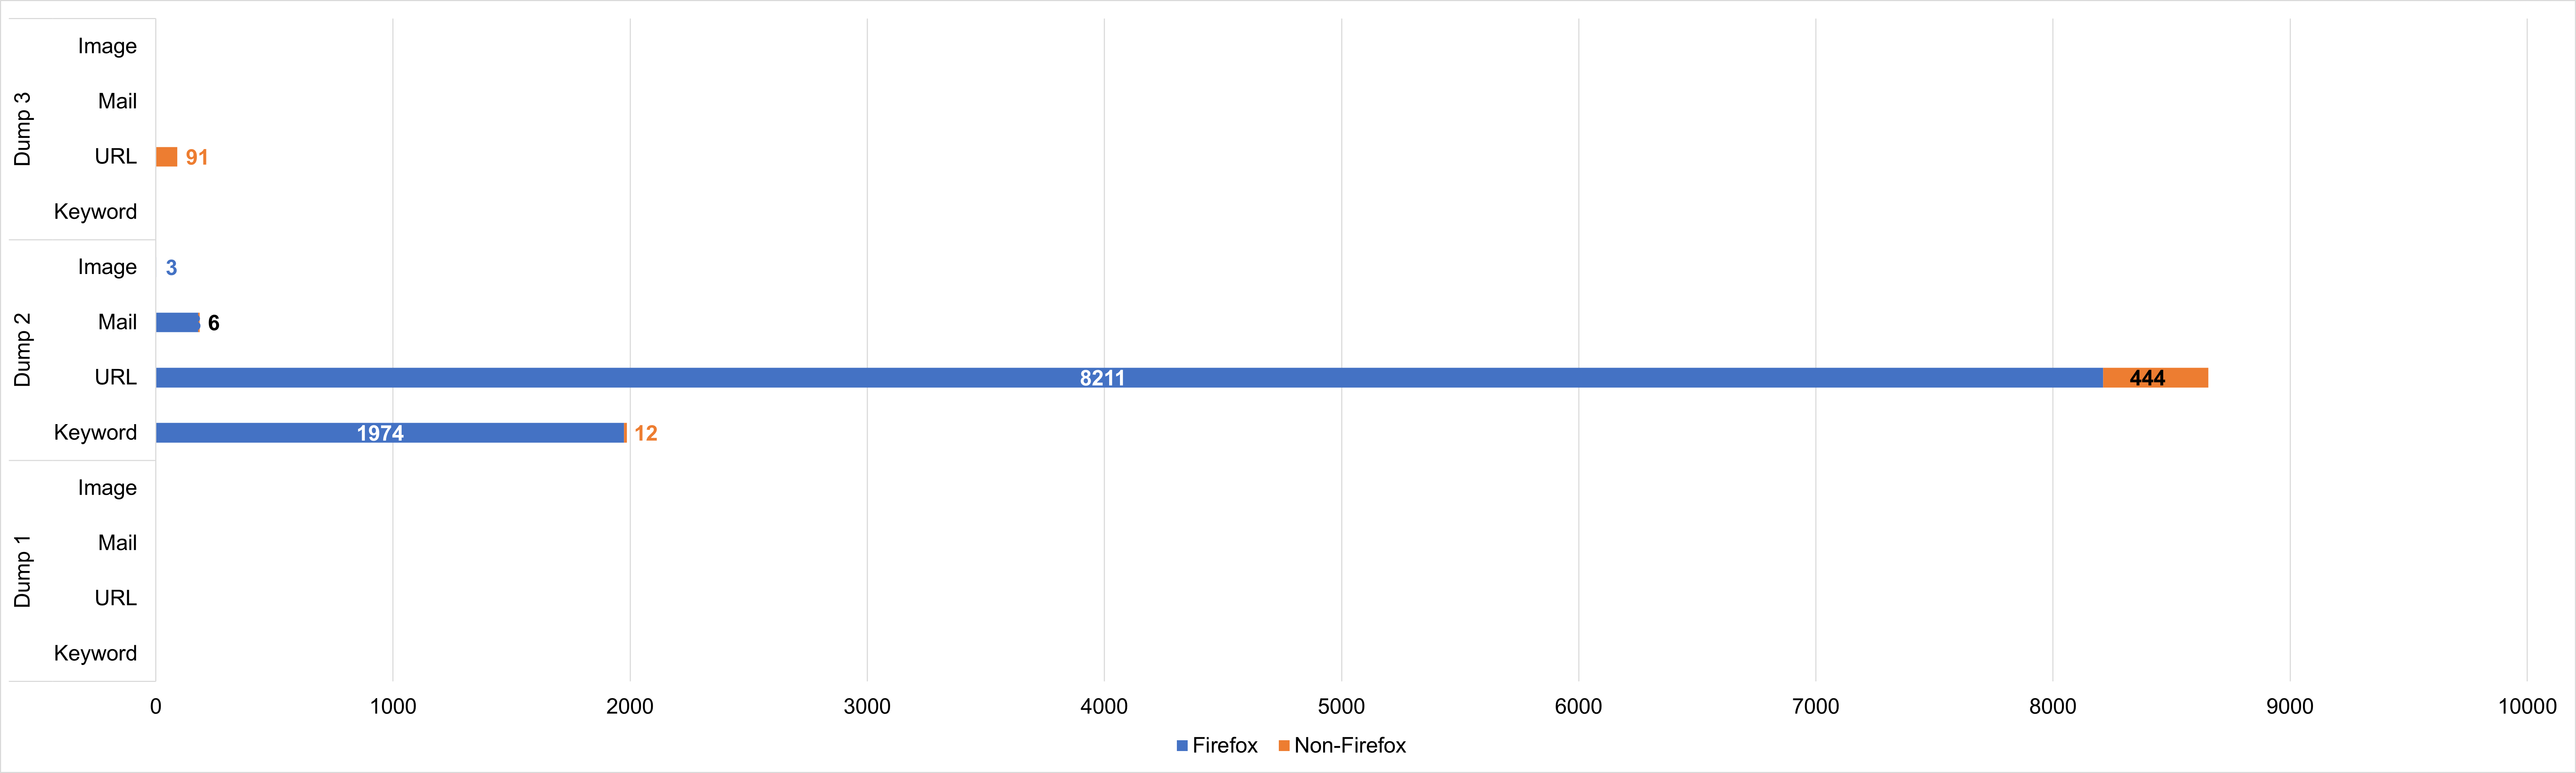
\includegraphics{bilder/volatility/firefox/summary.png}}}
%	\label{chart:final-criteria}  
%	\caption{Summary}
%\end{figure}

\subsection*{Registry}
\label{subsection:ergebnisse-firefox-registry}
Die Analyse der Registry zählt gemäß Methodik in Kapitel \ref{subsection:methodik-datenanalyse-registry} sowohl zu den Common als auch Uncommon Locations. Weder in den Process Monitor ``SetValue`` Operations noch in den System- und User-Hives konnten PB Artefakte gefunden werden. Eine detaillierte Analyse dieser Common- und Uncommon Locations der Registry ist im Anhang X beschrieben.


%*** TODO: Zusammenfassung Firefox ***


\newpage


% ######################################################################
% ######################################################################
% ######################################################################
% ######################################################################


\section{Tor}

In diesem Abschnitt werden die Ergebnisse der Datenanalyse der Common Locations, Uncommon Locations sowie der Registry für den Tor-Browser präsentiert.

\subsection*{Common Locations}
Als Erstes werden die Common Locations analysiert, um potenzielle Hinweise auf Internetaktivitäten des Browsing Szenarios zu finden. Bei der Untersuchung der gängigen Speicherorte wurde gemäß der im Kapitel \ref{subsection:methodik-datenanalyse-commonlocations} beschriebenen Methodik zwischen Schreibvorgängen in den Protokolldateien des Process Monitors und den SQLite-Datenbanken zur Verwaltung von Benutzerdaten unterschieden. Dabei konnten in keiner Datei PB Artefakte gefunden werden. Eine detaillierte Analyse der Process Monitor ``WriteFile`` Operations sowie SQLite-Datenbänken ist im Anhang X beschrieben.

\subsection*{Uncommon Locations}
Nachfolgend werden die Analyseergebnisse der Tor Uncommon Locations beschrieben.
Dazu werden die vollständigen Speicherabbilder nach PB Artefakten untersucht ohne das genaue Browserverhalten zu berücksichtigen. Stattdessen wird sich auf die Vollständigkeit der Funktionen der Forensik-Tools Autopsy und Volatility verlassen.

\subsubsection*{Analyse mit Autopsy}

Im ersten Schritt wird Autopsy als konkretes forensisches Werkzeug verwendet, statt nur nur zur Dateiextraktion, wie es bei den Common Locations der Fall war.

Eine Stichwortsuche in Autopsy in allen fünft Festplatten-Images nach PB Artefakten ergab keine Treffer.

Ebenso wurden in den von automatisch kategorisierten Dateien kein PB Artefakte gefunden. 
Im Anhang \ref{subsubsection:appendix-tor-uncommon-locations-autopsy} ist eine detaillierte Analyse der kategorisierten Dateien beschrieben.


\subsubsection*{Analyse mit Volatility}

Nachfolgend werden die Ergebnisse der Analyse des RAMs mithilfe des Volatility Plugins Yarascan beschrieben. Die Yara-Regeln sind im Anhang \ref{appendix:yara-regeln} aufgelistet.

\paragraph*{Yara-Regel ``HTML``}
Wie bei Firefox konnten keine HTML Artefakte im RAM gefunden werden. Deshalb wird diese Kategorie nicht aufgeführt.

\paragraph*{Yara-Regel ``Suchbegriffe``}
Wie in Abbildung \ref{chart:tor-volatility-keywords} gezeigt, wurden ausschließlich während des Browsing-Szenarios (RAM-Dump 2) und nach Erstellen einer ``Neuen Identität`` (RAM Dump 3-1) Suchbegriffe des Browsing-Szenarios gefunden.
Nachdem eine ``Neue Identität`` erstellt wurde reduzierten sich die gefundenen Artefakte deutlich. 
Die Suchbegriffe wurden hauptsächlich in Firefox Prozessen gefunden. Kein Artefakt war im Tor.exe Prozess zu finden.
Mit 4833 Artefakten wurden am häufigsten ``pfaffenhofen`` nach dem Browsing Szenario im zweiten RAM-Dump gefunden. 
Nach dem Schließen des Tor-Browsers wurde keine Suchbegriffe mehr im RAM identifiziert.

\begin{table}[h!]
	\resizebox{\linewidth}{!}{
	\begin{tabular}{l}	
		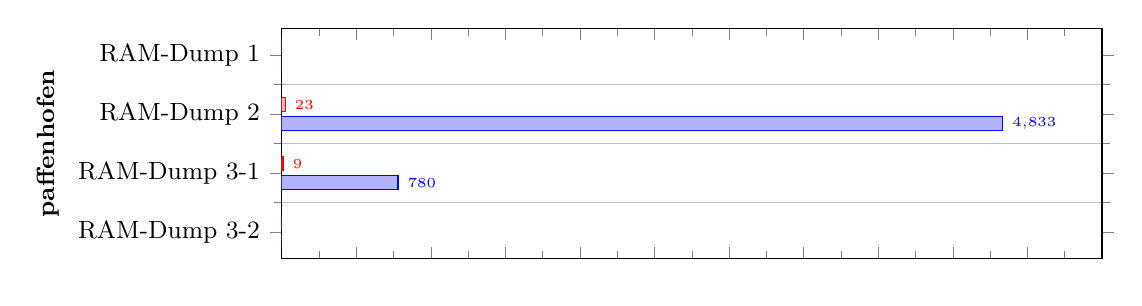
\begin{tikzpicture}
			\begin{axis}[
			xbar,
			width=12cm, 
			height=3cm, 
			ylabel style={align=center}, ylabel=\textbf{paffenhofen},
			y=0.75cm,
			symbolic y coords={RAM-Dump 3-2, RAM-Dump 3-1, RAM-Dump 2, RAM-Dump 1},
			label style={font=\small},
			tick label style={font=\small},
			ytick=data,
			xticklabels={,,},
            xmin = 0,
            xmax = 5500,
			nodes near coords, 
			nodes near coords align={horizontal},
			nodes near coords style={font=\tiny},
   			nodes near coords={\pgfmathfloatifflags{\pgfplotspointmeta}{0}{}{\pgfmathprintnumber{\pgfplotspointmeta}}},
			bar width=.17cm,
			enlarge y limits={abs=2*\pgfplotbarwidth},
			scaled x ticks=false,
			legend style={
				at={(0.5,-0.1)},
				anchor=north
			},
			legend columns=3,
    		yminorgrids = true,minor tick num=1
			]
				\addplot coordinates {
				(0,RAM-Dump 3-2)  (780,RAM-Dump 3-1) (4833,RAM-Dump 2) (0,RAM-Dump 1)
				};
%				\addplot coordinates {
%				(0,RAM-Dump 3-2)  (0,RAM-Dump 3-1) (0,RAM-Dump 2) (0,RAM-Dump 1)
%				};
				\addplot coordinates {
				(0,RAM-Dump 3-2)  (9,RAM-Dump 3-1) (23,RAM-Dump 2) (0,RAM-Dump 1)
				};
%				\legend{firefox.exe, tor.exe, Andere Prozesse}
			\end{axis}
		\end{tikzpicture}
		\\[-7pt]
		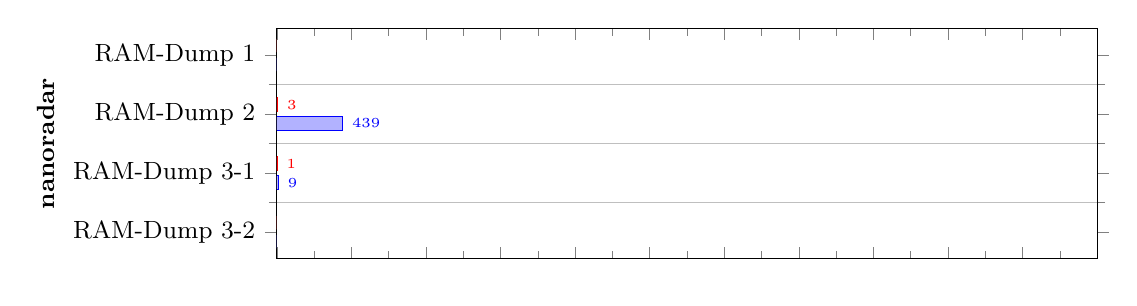
\begin{tikzpicture}
			\begin{axis}[
			xbar,
			width=12cm, 
			height=3cm, 
			ylabel style={align=center}, ylabel=\textbf{nanoradar},
			y=0.75cm,
			symbolic y coords={RAM-Dump 3-2, RAM-Dump 3-1, RAM-Dump 2, RAM-Dump 1},
			label style={font=\small},
			tick label style={font=\small},
			ytick=data,
			xticklabels={,,},
            xmin = 0,
            xmax = 5500,
			nodes near coords, 
			nodes near coords align={horizontal},
			nodes near coords style={font=\tiny},
   			nodes near coords={\pgfmathfloatifflags{\pgfplotspointmeta}{0}{}{\pgfmathprintnumber{\pgfplotspointmeta}}},
			bar width=.17cm,
			enlarge y limits={abs=2*\pgfplotbarwidth},
			scaled x ticks=false,
			legend style={
				at={(0.5,-0.1)},
				anchor=north
			},
			legend columns=3,
    		yminorgrids = true,minor tick num=1
			]
				\addplot coordinates {
				(0,RAM-Dump 3-2)  (9,RAM-Dump 3-1) (439,RAM-Dump 2) (0,RAM-Dump 1)
				};
%				\addplot coordinates {
%				(0,RAM-Dump 3-2)  (0,RAM-Dump 3-1) (0,RAM-Dump 2) (0,RAM-Dump 1)
%				};
				\addplot coordinates {
				(0,RAM-Dump 3-2)  (1,RAM-Dump 3-1) (3,RAM-Dump 2) (0,RAM-Dump 1)
				};
%				\legend{firefox.exe, tor.exe, Andere Prozesse}
			\end{axis}
		\end{tikzpicture}
		\\[-7pt]
		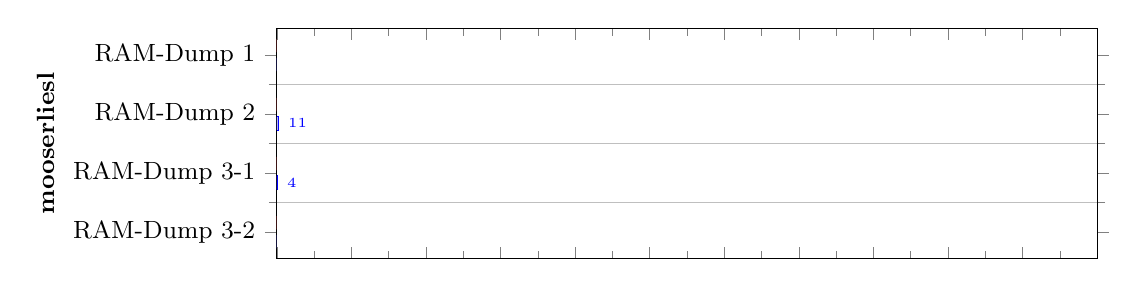
\begin{tikzpicture}
			\begin{axis}[
			xbar,
			width=12cm, 
			height=3cm, 
			ylabel style={align=center}, ylabel=\textbf{mooserliesl},
			y=0.75cm,
			symbolic y coords={RAM-Dump 3-2, RAM-Dump 3-1, RAM-Dump 2, RAM-Dump 1},
			label style={font=\small},
			tick label style={font=\small},
			ytick=data,
			xticklabels={,,},
            xmin = 0,
            xmax = 5500,
			nodes near coords, 
			nodes near coords align={horizontal},
			nodes near coords style={font=\tiny},
   			nodes near coords={\pgfmathfloatifflags{\pgfplotspointmeta}{0}{}{\pgfmathprintnumber{\pgfplotspointmeta}}},
			bar width=.17cm,
			enlarge y limits={abs=2*\pgfplotbarwidth},
			scaled x ticks=false,
			legend style={
				at={(0.5,-0.1)},
				anchor=north
			},
			legend columns=3,
    		yminorgrids = true,minor tick num=1
			]
				\addplot coordinates {
				(0,RAM-Dump 3-2)  (4,RAM-Dump 3-1) (11,RAM-Dump 2) (0,RAM-Dump 1)
				};
%				\addplot coordinates {
%				(0,RAM-Dump 3-2)  (0,RAM-Dump 3-1) (0,RAM-Dump 2) (0,RAM-Dump 1)
%				};
				\addplot coordinates {
				(0,RAM-Dump 3-2)  (0,RAM-Dump 3-1) (0,RAM-Dump 2) (0,RAM-Dump 1)
				};
%				\legend{firefox.exe, tor.exe, Andere Prozesse}
			\end{axis}
		\end{tikzpicture}
		\\[-7pt]
		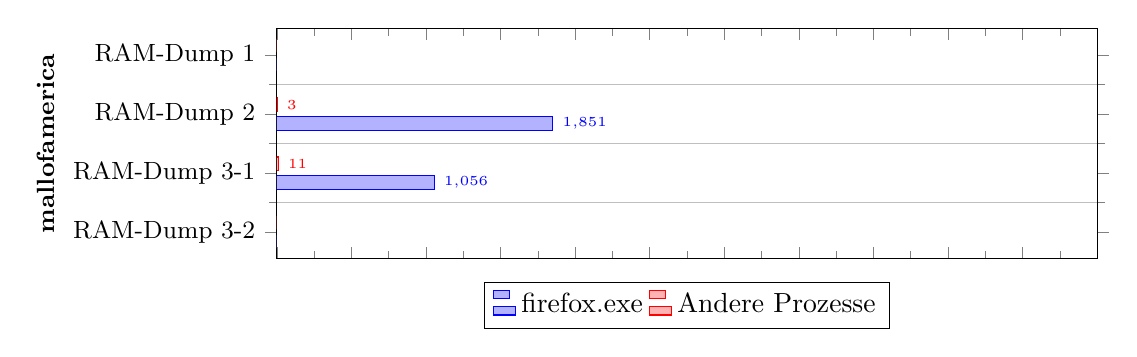
\begin{tikzpicture}
			\begin{axis}[
			xbar,
			width=12cm, 
			height=3cm, 
			ylabel style={align=center}, ylabel=\textbf{mallofamerica},
			y=0.75cm,
			symbolic y coords={RAM-Dump 3-2, RAM-Dump 3-1, RAM-Dump 2, RAM-Dump 1},
			label style={font=\small},
			tick label style={font=\small},
			ytick=data,
			xticklabels={,,},
            xmin = 0,
            xmax = 5500,
			nodes near coords, 
			nodes near coords align={horizontal},
			nodes near coords style={font=\tiny},
   			nodes near coords={\pgfmathfloatifflags{\pgfplotspointmeta}{0}{}{\pgfmathprintnumber{\pgfplotspointmeta}}},
			bar width=.17cm,
			enlarge y limits={abs=2*\pgfplotbarwidth},
			scaled x ticks=false,
			legend style={
				at={(0.5,-0.1)},
				anchor=north
			},
			legend columns=3,
    		yminorgrids = true,minor tick num=1
			]
				\addplot coordinates {
				(0,RAM-Dump 3-2)  (1056,RAM-Dump 3-1) (1851,RAM-Dump 2) (0,RAM-Dump 1)
				};
%				\addplot coordinates {
%				(0,RAM-Dump 3-2)  (0,RAM-Dump 3-1) (0,RAM-Dump 2) (0,RAM-Dump 1)
%				};
				\addplot coordinates {
				(0,RAM-Dump 3-2)  (11,RAM-Dump 3-1) (3,RAM-Dump 2) (0,RAM-Dump 1)
				};
				\legend{firefox.exe, Andere Prozesse}
			\end{axis}
		\end{tikzpicture}
	\end{tabular}
	}
	\caption{Gefundene Suchbegriffe im Tor RAM}
	\label{chart:tor-volatility-keywords}
\end{table}
%\begin{figure}[h!]
%	\centerline{\resizebox{\linewidth}{!}{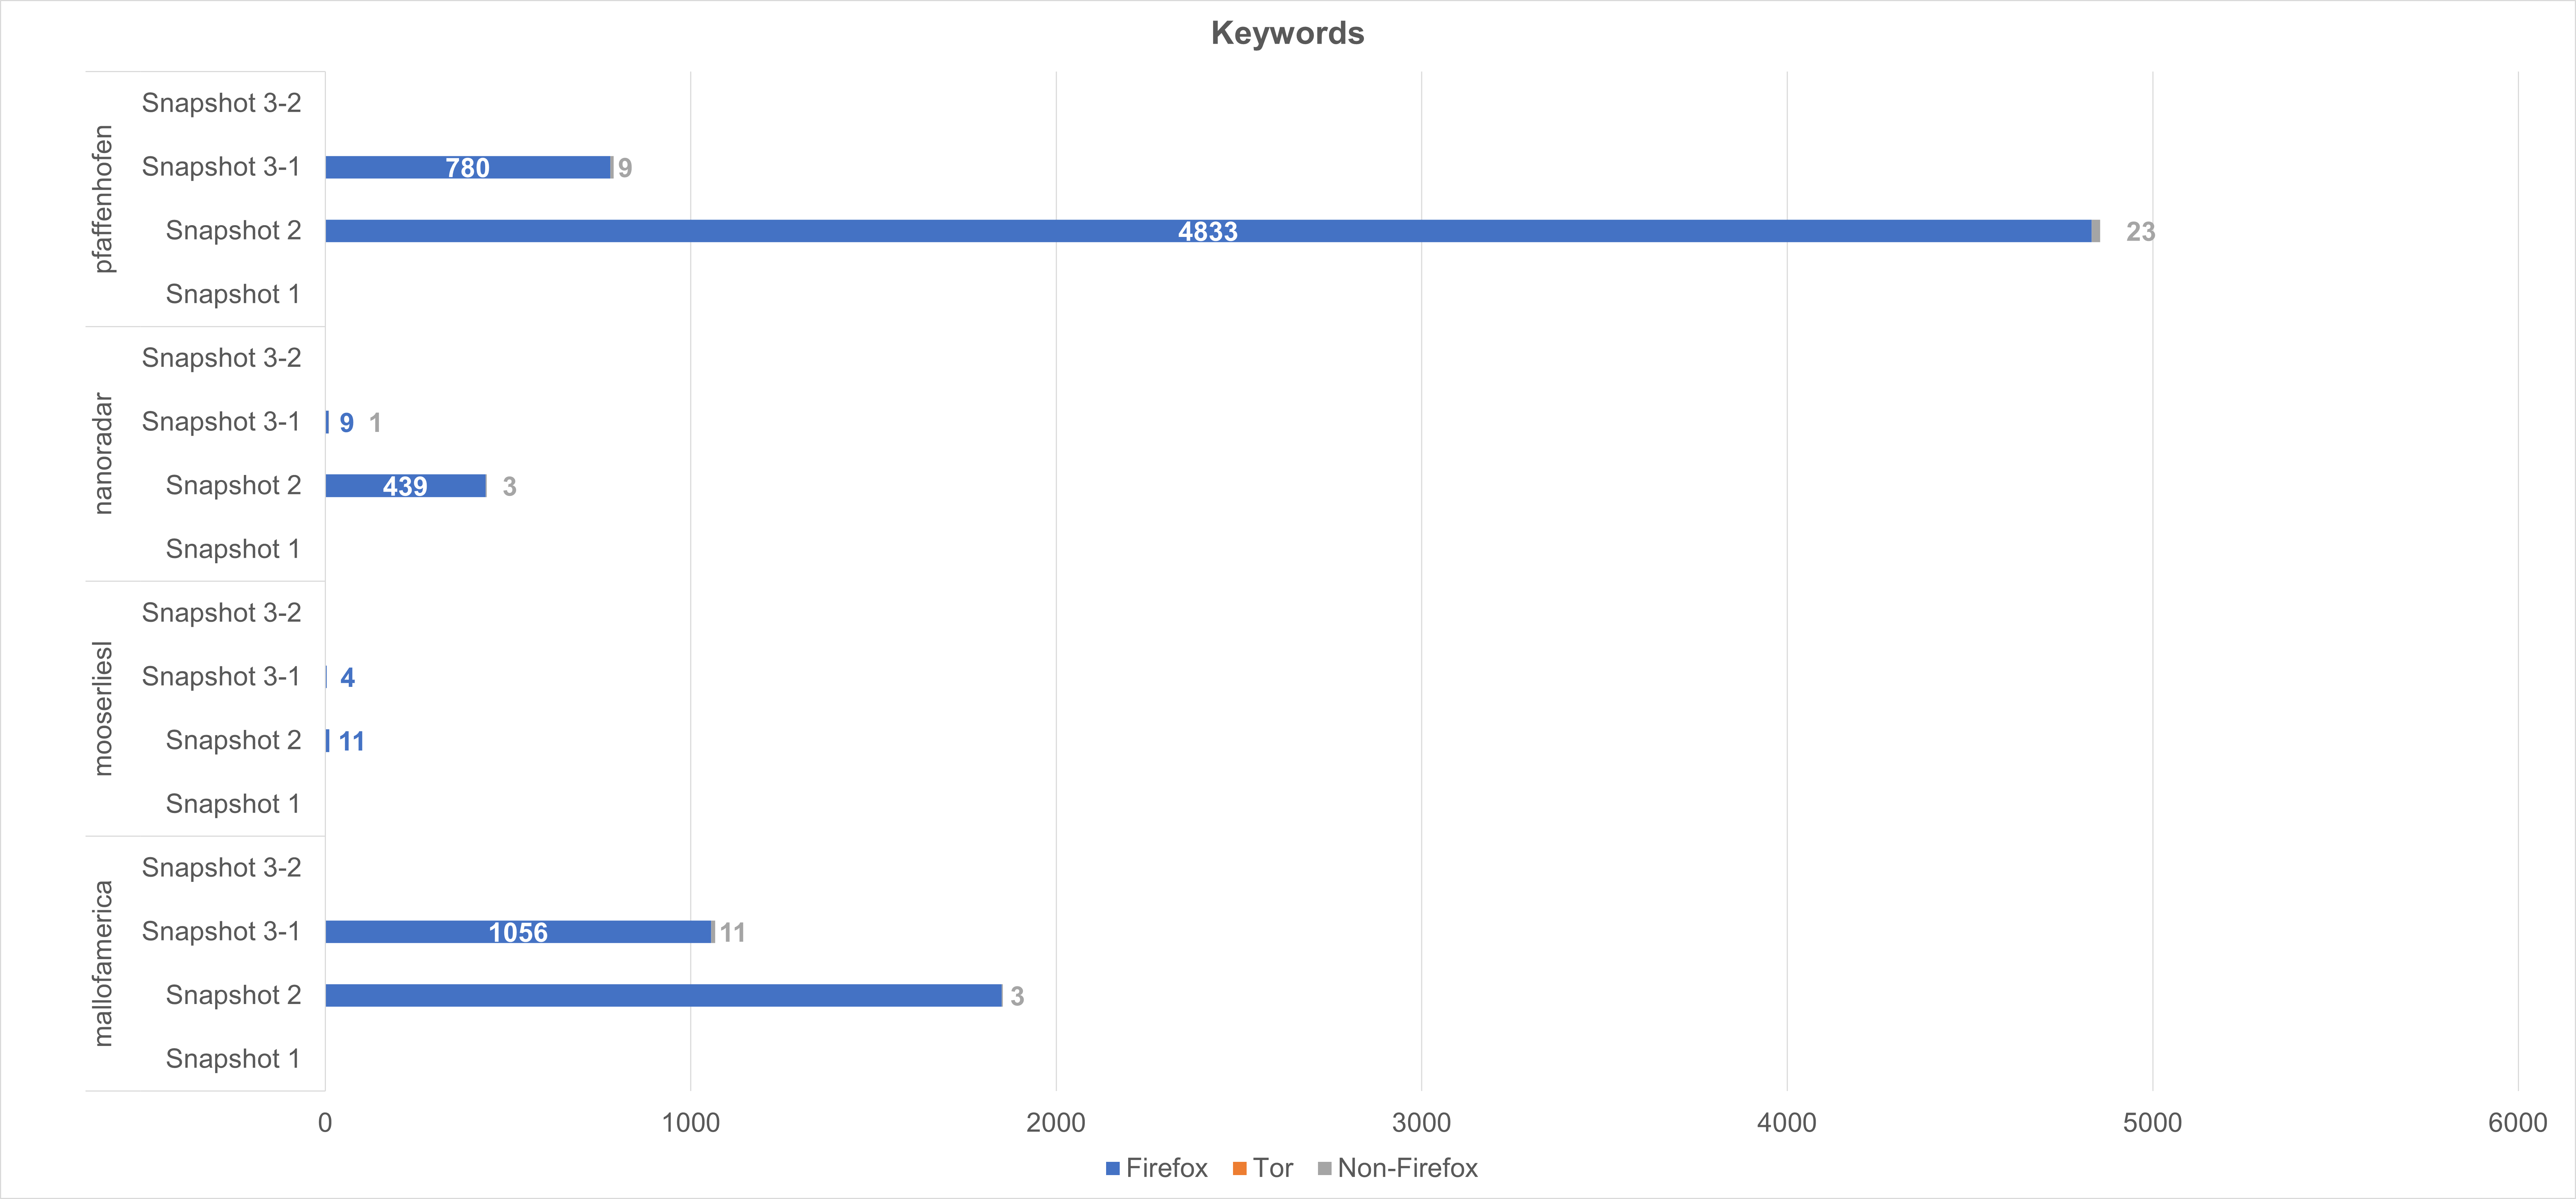
\includegraphics{bilder/volatility/tor/keywords.png}}}
%	\label{chart:final-criteria}  
%	\caption{Keywords}
%\end{figure}

\paragraph*{Yara-Regel ``URLs``}
Wie bei der Yara-Regel ``Suchbegriffe`` wurden wie in Abbildung \ref{chart:tor-volatility-urls} gezeigt, ausschließlich während des Browsing-Szenarios (RAM-Dump 2) und nach Zuweisung einer neuen Identität (RAM-Dump 3-1) URL Artefakte gefunden. Ebenso wurden im RAM Dump 3-1 bei deutlich weniger Artefakte URLs als in RAM Dump 2 gefunden. 
Für diese Yara-Regel wurden nach Firefox-Prozessen hauptsächlich Artefakt in Tor-Prozessen gefunden. Am wenigsten Artefakte waren in anderen Prozessen zu finden.
Auffällig ist, dass die URL ``mallofamerica.com`` 26.505 mal in RAM-Dump 2 gefunden wurde. Im Gegensatz dazu wurde ``mooserliesl.de`` nur 508 mal im zweiten RAM Dump  gefunden. Nach Schließen des Tor-Browsers wurden keine URL Artefakte mehr im RAM gefunden.
\begin{table}[h!]
	\resizebox{\linewidth}{!}{
	\begin{tabular}{l}	
		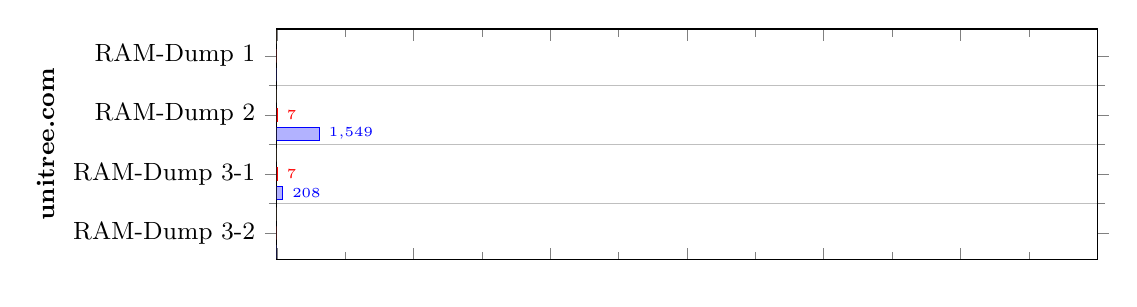
\begin{tikzpicture}
			\begin{axis}[
			xbar,
			width=12cm, 
			height=3cm, 
			ylabel style={align=center}, ylabel=\textbf{unitree.com},
			y=0.75cm,
			symbolic y coords={RAM-Dump 3-2, RAM-Dump 3-1, RAM-Dump 2, RAM-Dump 1},
			label style={font=\small},
			tick label style={font=\small},
			ytick=data,
			xticklabels={,,},
            xmin = 0,
            xmax = 30000,
			nodes near coords, 
			nodes near coords align={horizontal},
			nodes near coords style={font=\tiny},
   			nodes near coords={\pgfmathfloatifflags{\pgfplotspointmeta}{0}{}{\pgfmathprintnumber{\pgfplotspointmeta}}},
			bar width=.17cm,
			enlarge y limits={abs=2*\pgfplotbarwidth},
			scaled x ticks=false,
			legend style={
				at={(0.5,-0.1)},
				anchor=north
			},
			legend columns=3,
    		yminorgrids = true,minor tick num=1
			]
				\addplot coordinates {
				(0,RAM-Dump 3-2)  (208,RAM-Dump 3-1) (1549,RAM-Dump 2) (0,RAM-Dump 1)
				};
				\addplot coordinates {
				(0,RAM-Dump 3-2)  (7,RAM-Dump 3-1) (7,RAM-Dump 2) (0,RAM-Dump 1)
				};
				\addplot coordinates {
				(0,RAM-Dump 3-2)  (0,RAM-Dump 3-1) (0,RAM-Dump 2) (0,RAM-Dump 1)
				};
%				\legend{firefox.exe, tor.exe, Andere Prozesse}
			\end{axis}
		\end{tikzpicture}
		\\[-7pt]
		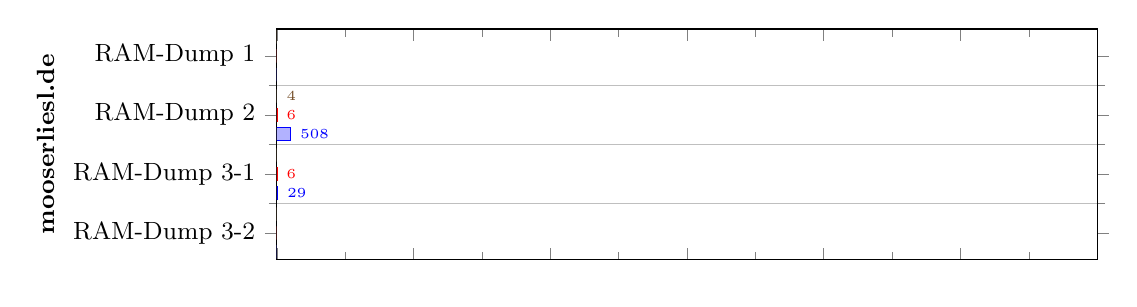
\begin{tikzpicture}
			\begin{axis}[
			xbar,
			width=12cm, 
			height=3cm, 
			ylabel style={align=center}, ylabel=\textbf{mooserliesl.de},
			y=0.75cm,
			symbolic y coords={RAM-Dump 3-2, RAM-Dump 3-1, RAM-Dump 2, RAM-Dump 1},
			label style={font=\small},
			tick label style={font=\small},
			ytick=data,
			xticklabels={,,},
            xmin = 0,
            xmax = 30000,
			nodes near coords, 
			nodes near coords align={horizontal},
			nodes near coords style={font=\tiny},
   			nodes near coords={\pgfmathfloatifflags{\pgfplotspointmeta}{0}{}{\pgfmathprintnumber{\pgfplotspointmeta}}},
			bar width=.17cm,
			enlarge y limits={abs=2*\pgfplotbarwidth},
			scaled x ticks=false,
			legend style={
				at={(0.5,-0.1)},
				anchor=north
			},
			legend columns=3,
    		yminorgrids = true,minor tick num=1
			]
				\addplot coordinates {
				(0,RAM-Dump 3-2)  (29,RAM-Dump 3-1) (508,RAM-Dump 2) (0,RAM-Dump 1)
				};
				\addplot coordinates {
				(0,RAM-Dump 3-2)  (6,RAM-Dump 3-1) (6,RAM-Dump 2) (0,RAM-Dump 1)
				};
				\addplot coordinates {
				(0,RAM-Dump 3-2)  (0,RAM-Dump 3-1) (4,RAM-Dump 2) (0,RAM-Dump 1)
				};
%				\legend{firefox.exe, tor.exe, Andere Prozesse}
			\end{axis}
		\end{tikzpicture}
		\\[-7pt]
		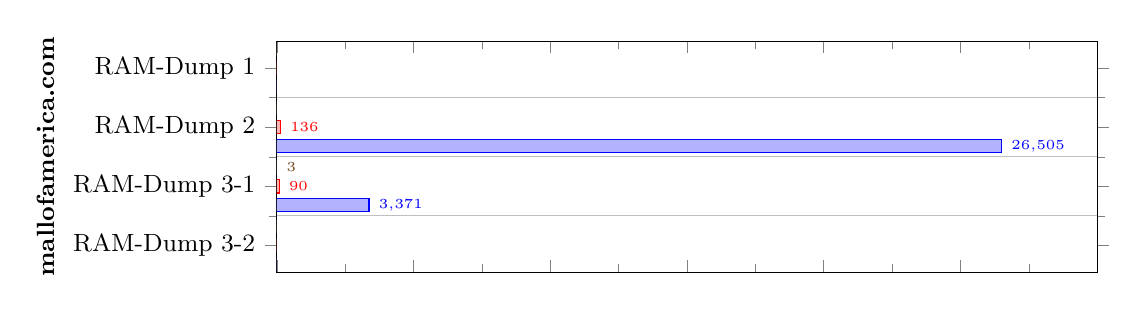
\begin{tikzpicture}
			\begin{axis}[
			xbar,
			width=12cm, 
			height=3cm, 
			ylabel style={align=center}, ylabel=\textbf{mallofamerica.com},
			y=0.75cm,
			symbolic y coords={RAM-Dump 3-2, RAM-Dump 3-1, RAM-Dump 2, RAM-Dump 1},
			label style={font=\small},
			tick label style={font=\small},
			ytick=data,
			xticklabels={,,},
            xmin = 0,
            xmax = 30000,
			nodes near coords, 
			nodes near coords align={horizontal},
			nodes near coords style={font=\tiny},
   			nodes near coords={\pgfmathfloatifflags{\pgfplotspointmeta}{0}{}{\pgfmathprintnumber{\pgfplotspointmeta}}},
			bar width=.17cm,
			enlarge y limits={abs=2*\pgfplotbarwidth},
			scaled x ticks=false,
			legend style={
				at={(0.5,-0.1)},
				anchor=north
			},
			legend columns=3,
    		yminorgrids = true,minor tick num=1
			]
				\addplot coordinates {
				(0,RAM-Dump 3-2)  (3371,RAM-Dump 3-1) (26505,RAM-Dump 2) (0,RAM-Dump 1)
				};
				\addplot coordinates {
				(0,RAM-Dump 3-2)  (90,RAM-Dump 3-1) (136,RAM-Dump 2) (0,RAM-Dump 1)
				};
				\addplot coordinates {
				(0,RAM-Dump 3-2)  (3,RAM-Dump 3-1) (0,RAM-Dump 2) (0,RAM-Dump 1)
				};
%				\legend{firefox.exe, tor.exe, Andere Prozesse}
			\end{axis}
		\end{tikzpicture}
		\\[-7pt]
		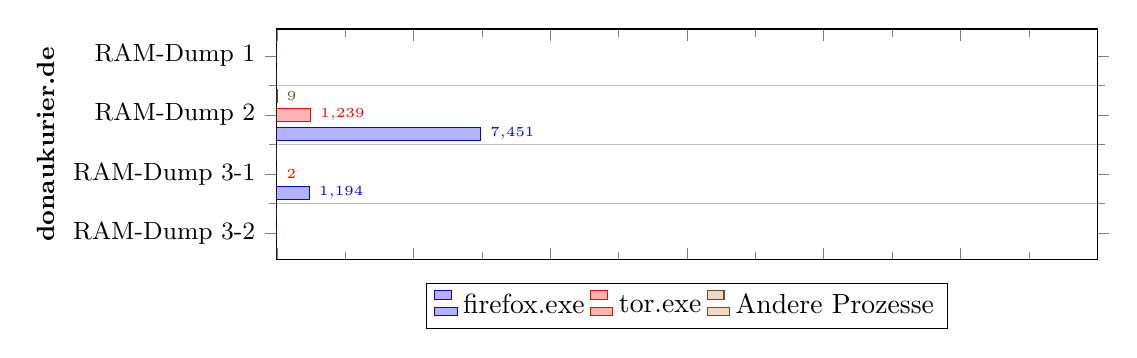
\begin{tikzpicture}
			\begin{axis}[
			xbar,
			width=12cm, 
			height=3cm, 
			ylabel style={align=center}, ylabel=\textbf{donaukurier.de},
			y=0.75cm,
			symbolic y coords={RAM-Dump 3-2, RAM-Dump 3-1, RAM-Dump 2, RAM-Dump 1},
			label style={font=\small},
			tick label style={font=\small},
			ytick=data,
			xticklabels={,,},
            xmin = 0,
            xmax = 30000,
			nodes near coords, 
			nodes near coords align={horizontal},
			nodes near coords style={font=\tiny},
   			nodes near coords={\pgfmathfloatifflags{\pgfplotspointmeta}{0}{}{\pgfmathprintnumber{\pgfplotspointmeta}}},
			bar width=.17cm,
			enlarge y limits={abs=2*\pgfplotbarwidth},
			scaled x ticks=false,
			legend style={
				at={(0.5,-0.1)},
				anchor=north
			},
			legend columns=3,
    		yminorgrids = true,minor tick num=1
			]
				\addplot coordinates {
				(0,RAM-Dump 3-2)  (1194,RAM-Dump 3-1) (7451,RAM-Dump 2) (0,RAM-Dump 1)
				};
				\addplot coordinates {
				(0,RAM-Dump 3-2)  (2,RAM-Dump 3-1) (1239,RAM-Dump 2) (0,RAM-Dump 1)
				};
				\addplot coordinates {
				(0,RAM-Dump 3-2)  (0,RAM-Dump 3-1) (9,RAM-Dump 2) (0,RAM-Dump 1)
				};
				\legend{firefox.exe, tor.exe, Andere Prozesse}
			\end{axis}
		\end{tikzpicture}
	\end{tabular}
	}
	\caption{Gefundene URLs im Tor RAM}
	\label{chart:tor-volatility-urls}
\end{table}
%\begin{figure}[h!]
%	\centerline{\resizebox{\linewidth}{!}{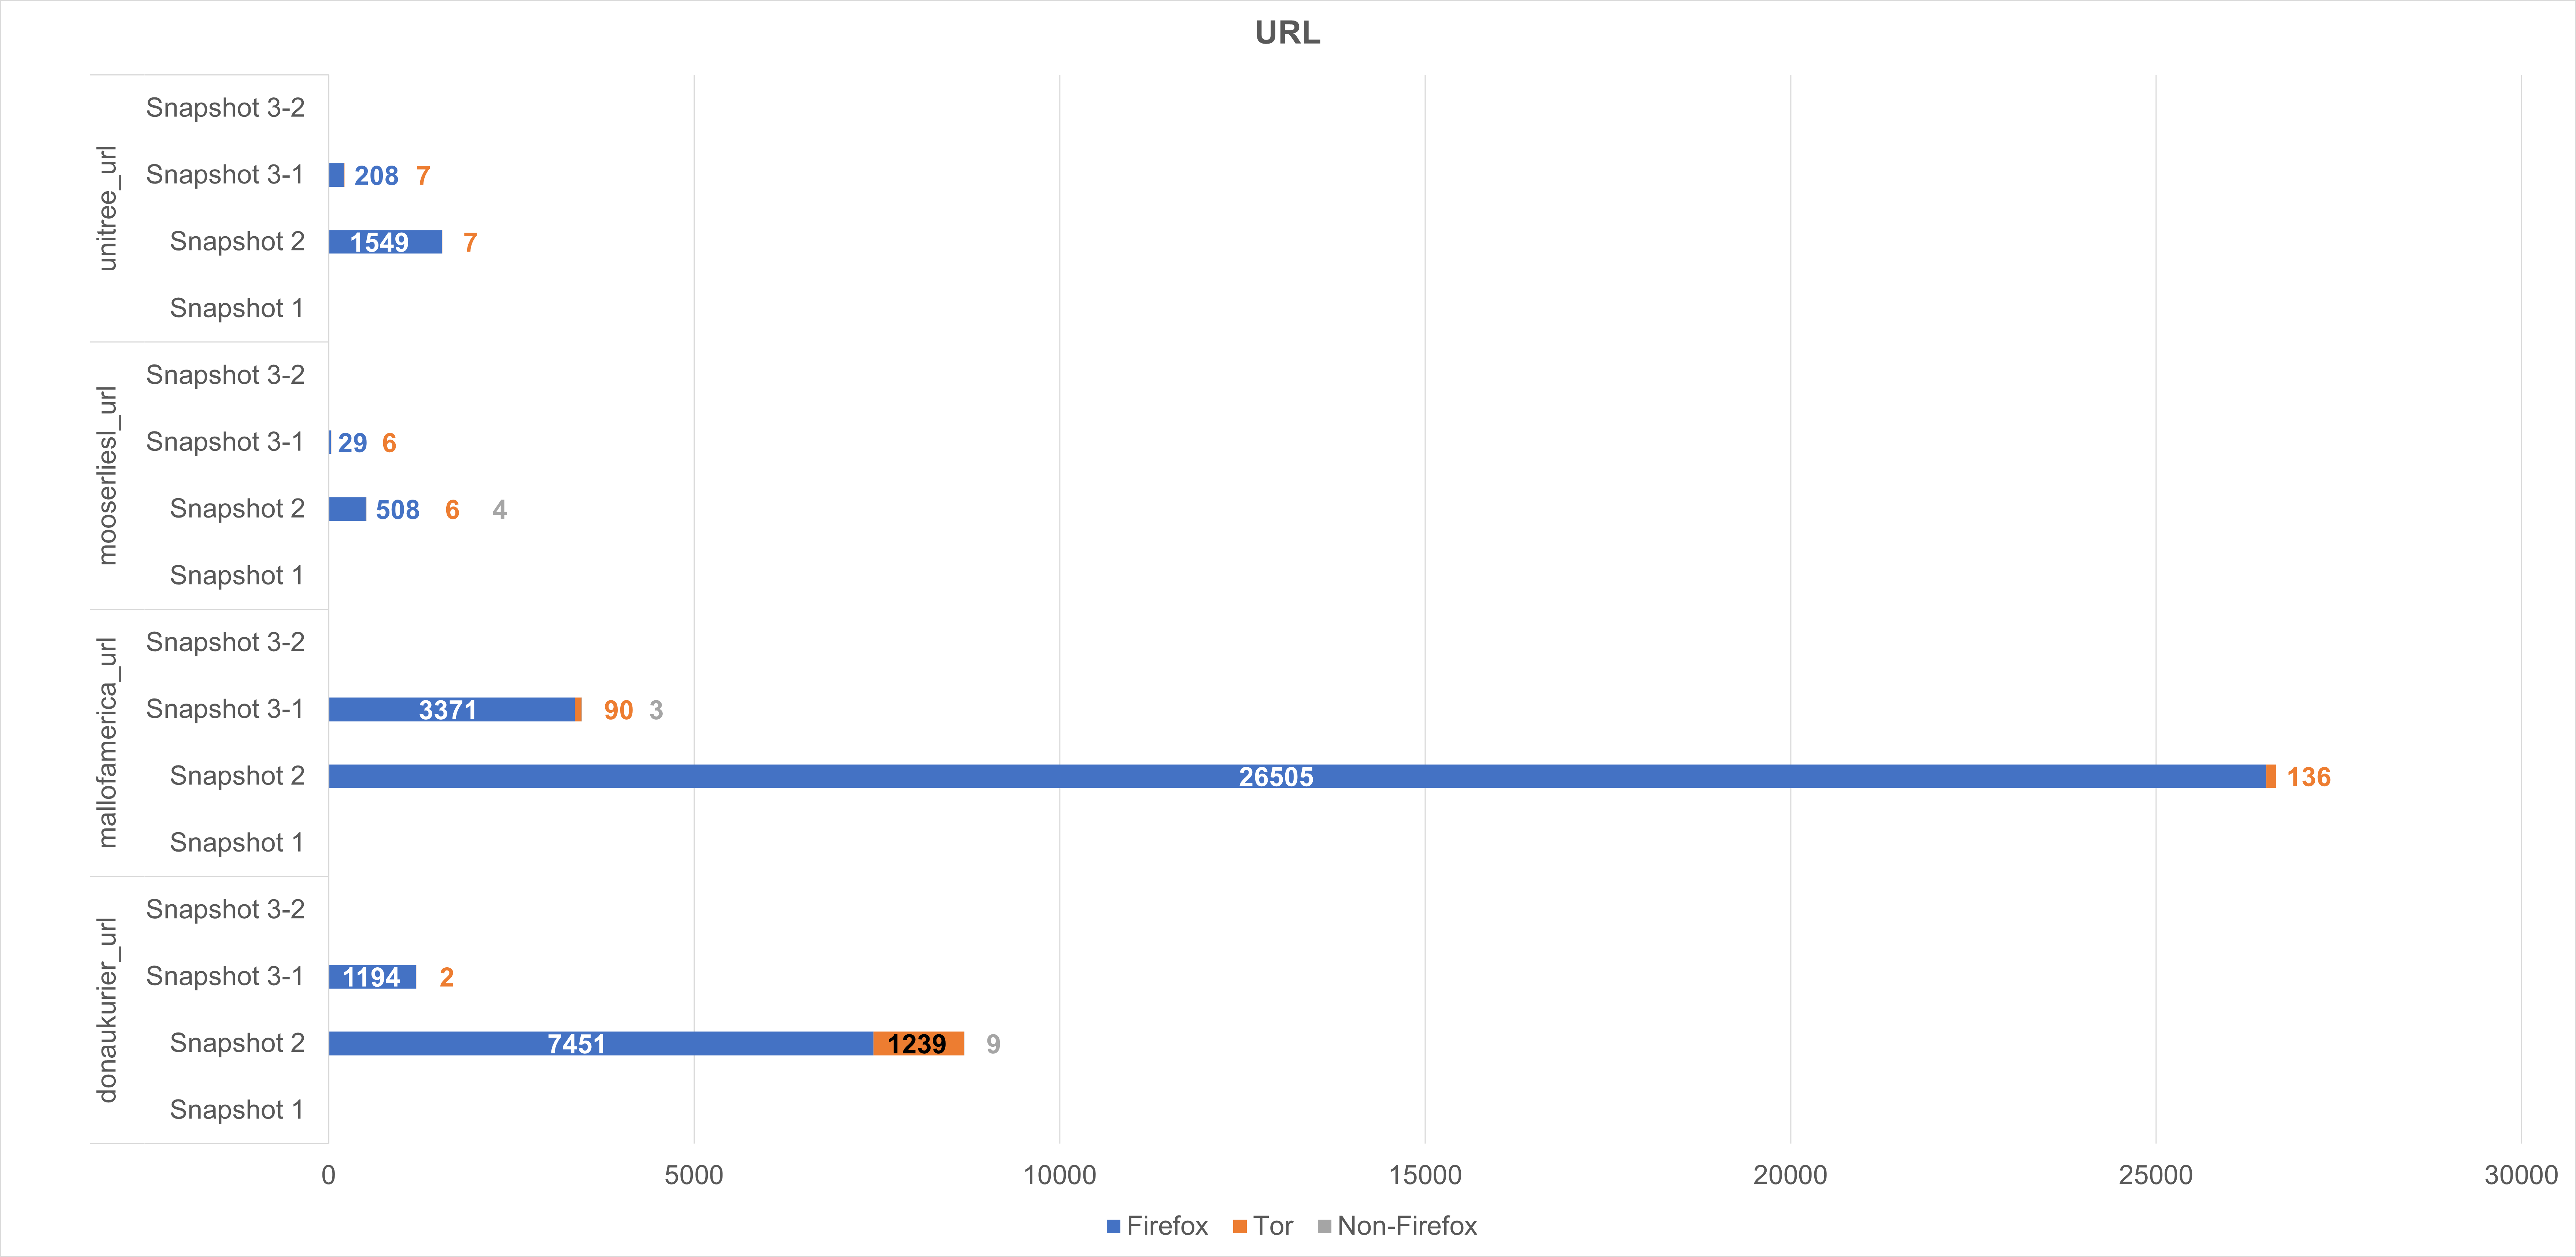
\includegraphics{bilder/volatility/tor/url.png}}}
%	\label{chart:final-criteria}  
%	\caption{URL}
%\end{figure}

\paragraph*{Yara-Regel ``E-Mail``}
Nach dem Browsing-Szenario, vor Zuweisung einer ``Neuen Identität`` (RAM-Dump 2) konnten alle Mail Artefakte gefunden werden.
\begin{table}[h!]
	\resizebox{\linewidth}{!}{
	\begin{tabular}{r}	
		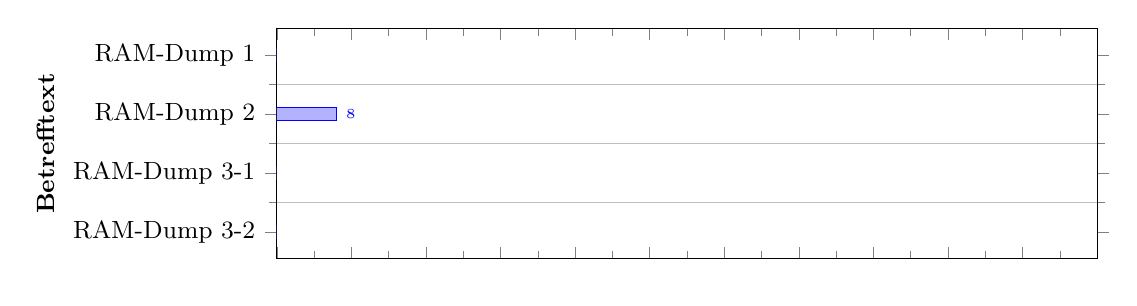
\begin{tikzpicture}					
			\begin{axis}[
			xbar,
			width=12cm, 
			height=3cm, 
			ylabel style={align=center}, ylabel=\textbf{Betrefftext},
			y=0.75cm,
			symbolic y coords={RAM-Dump 3-2, RAM-Dump 3-1, RAM-Dump 2, RAM-Dump 1},
			label style={font=\small},
			tick label style={font=\small},
			ytick=data,
			xticklabels={,,},
            xmin = 0,
            xmax = 110,
			nodes near coords, 
			nodes near coords align={horizontal},
			nodes near coords style={font=\tiny},
   			nodes near coords={\pgfmathfloatifflags{\pgfplotspointmeta}{0}{}{\pgfmathprintnumber{\pgfplotspointmeta}}},
			bar width=.17cm,
			enlarge y limits={abs=2*\pgfplotbarwidth},
			scaled x ticks=false,
			legend style={
				at={(0.5,-0.1)},
				anchor=north
			},
			legend columns=3,
    		yminorgrids = true,minor tick num=1
			]
				\addplot coordinates {
				(0,RAM-Dump 3-2)  (0,RAM-Dump 3-1) (8,RAM-Dump 2) (0,RAM-Dump 1)
				};
%				\addplot coordinates {
%				(0,RAM-Dump 3-2)  (0,RAM-Dump 3-1) (0,RAM-Dump 2) (0,RAM-Dump 1)
%				};
%				\addplot coordinates {
%				(0,RAM-Dump 3-2)  (0,RAM-Dump 3-1) (0,RAM-Dump 2) (0,RAM-Dump 1)
%				};
%				\legend{firefox.exe, tor.exe, Andere Prozesse}
			\end{axis}
		\end{tikzpicture}
		\\[-7pt]
		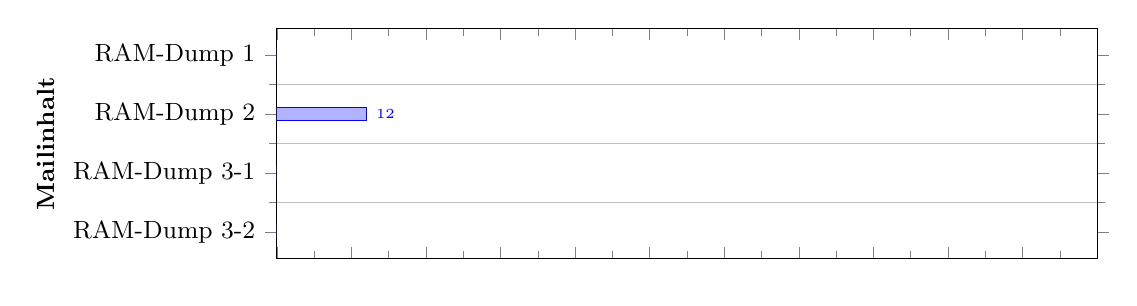
\begin{tikzpicture}
			\begin{axis}[
			xbar,
			width=12cm, 
			height=3cm, 
			ylabel style={align=center}, ylabel=\textbf{Mailinhalt},
			y=0.75cm,
			symbolic y coords={RAM-Dump 3-2, RAM-Dump 3-1, RAM-Dump 2, RAM-Dump 1},
			label style={font=\small},
			tick label style={font=\small},
			ytick=data,
			xticklabels={,,},
            xmin = 0,
            xmax = 110,
			nodes near coords, 
			nodes near coords align={horizontal},
			nodes near coords style={font=\tiny},
   			nodes near coords={\pgfmathfloatifflags{\pgfplotspointmeta}{0}{}{\pgfmathprintnumber{\pgfplotspointmeta}}},
			bar width=.17cm,
			enlarge y limits={abs=2*\pgfplotbarwidth},
			scaled x ticks=false,
			legend style={
				at={(0.5,-0.1)},
				anchor=north
			},
			legend columns=3,
    		yminorgrids = true,minor tick num=1
			]
				\addplot coordinates {
				(0,RAM-Dump 3-2)  (0,RAM-Dump 3-1) (12,RAM-Dump 2) (0,RAM-Dump 1)
				};
%				\addplot coordinates {
%				(0,RAM-Dump 3-2)  (0,RAM-Dump 3-1) (0,RAM-Dump 2) (0,RAM-Dump 1)
%				};
%				\addplot coordinates {
%				(0,RAM-Dump 3-2)  (0,RAM-Dump 3-1) (0,RAM-Dump 2) (0,RAM-Dump 1)
%				};
%				\legend{firefox.exe, tor.exe, Andere Prozesse}
			\end{axis}
		\end{tikzpicture}
		\\[-7pt]
		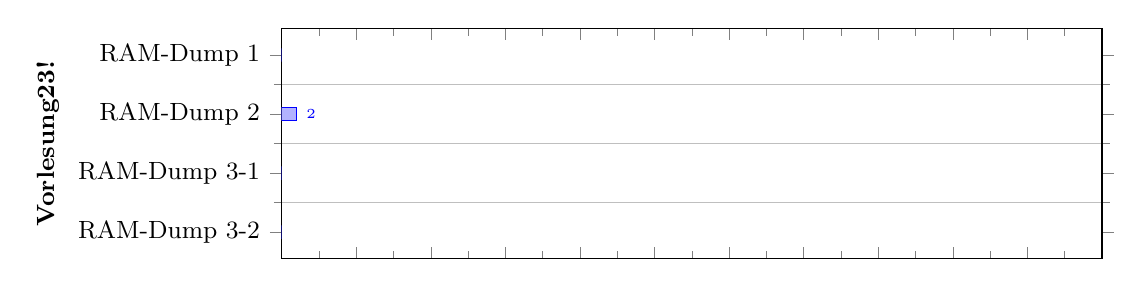
\begin{tikzpicture}
			\begin{axis}[
			xbar,
			width=12cm, 
			height=3cm, 
			ylabel style={align=center}, ylabel=\textbf{Vorlesung23!},
			y=0.75cm,
			symbolic y coords={RAM-Dump 3-2, RAM-Dump 3-1, RAM-Dump 2, RAM-Dump 1},
			label style={font=\small},
			tick label style={font=\small},
			ytick=data,
			xticklabels={,,},
            xmin = 0,
            xmax = 110,
			nodes near coords, 
			nodes near coords align={horizontal},
			nodes near coords style={font=\tiny},
   			nodes near coords={\pgfmathfloatifflags{\pgfplotspointmeta}{0}{}{\pgfmathprintnumber{\pgfplotspointmeta}}},
			bar width=.17cm,
			enlarge y limits={abs=2*\pgfplotbarwidth},
			scaled x ticks=false,
			legend style={
				at={(0.5,-0.1)},
				anchor=north
			},
			legend columns=3,
    		yminorgrids = true,minor tick num=1
			]
				\addplot coordinates {
				(0,RAM-Dump 3-2)  (0,RAM-Dump 3-1) (2,RAM-Dump 2) (0,RAM-Dump 1)
				};
%				\addplot coordinates {
%				(0,RAM-Dump 3-2)  (0,RAM-Dump 3-1) (0,RAM-Dump 2) (0,RAM-Dump 1)
%				};
%				\addplot coordinates {
%				(0,RAM-Dump 3-2)  (0,RAM-Dump 3-1) (0,RAM-Dump 2) (0,RAM-Dump 1)
%				};
%				\legend{firefox.exe, tor.exe, Andere Prozesse}
			\end{axis}
		\end{tikzpicture}
		\\[-8pt]
		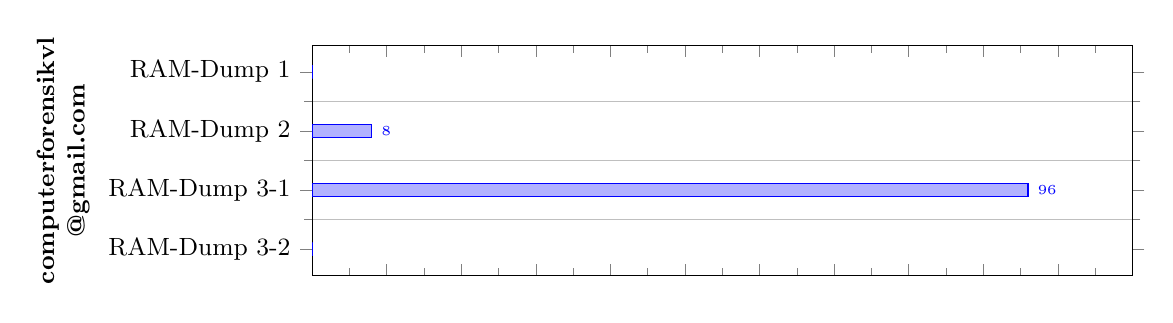
\begin{tikzpicture}
			\begin{axis}[
			xbar,
			width=12cm, 
			height=3cm, 
			ylabel style={align=center}, ylabel=\textbf{computerforensikvl}\\\textbf{@gmail.com},
			y=0.75cm,
			symbolic y coords={RAM-Dump 3-2, RAM-Dump 3-1, RAM-Dump 2, RAM-Dump 1},
			label style={font=\small},
			tick label style={font=\small},
			ytick=data,
			xticklabels={,,},
            xmin = 0,
            xmax = 110,
			nodes near coords, 
			nodes near coords align={horizontal},
			nodes near coords style={font=\tiny},
   			nodes near coords={\pgfmathfloatifflags{\pgfplotspointmeta}{0}{}{\pgfmathprintnumber{\pgfplotspointmeta}}},
			bar width=.17cm,
			enlarge y limits={abs=2*\pgfplotbarwidth},
			scaled x ticks=false,
			legend style={
				at={(0.5,-0.1)},
				anchor=north
			},
			legend columns=3,
    		yminorgrids = true,minor tick num=1
			]
				\addplot coordinates {
				(0,RAM-Dump 3-2)  (96,RAM-Dump 3-1) (8,RAM-Dump 2) (0,RAM-Dump 1)
				};
%				\addplot coordinates {
%				(0,RAM-Dump 3-2)  (0,RAM-Dump 3-1) (0,RAM-Dump 2) (0,RAM-Dump 1)
%				};
%				\addplot coordinates {
%				(0,RAM-Dump 3-2)  (0,RAM-Dump 3-1) (0,RAM-Dump 2) (0,RAM-Dump 1)
%				};
%				\legend{firefox.exe, tor.exe, Andere Prozesse}
			\end{axis}
		\end{tikzpicture}
		\\[-7pt]
		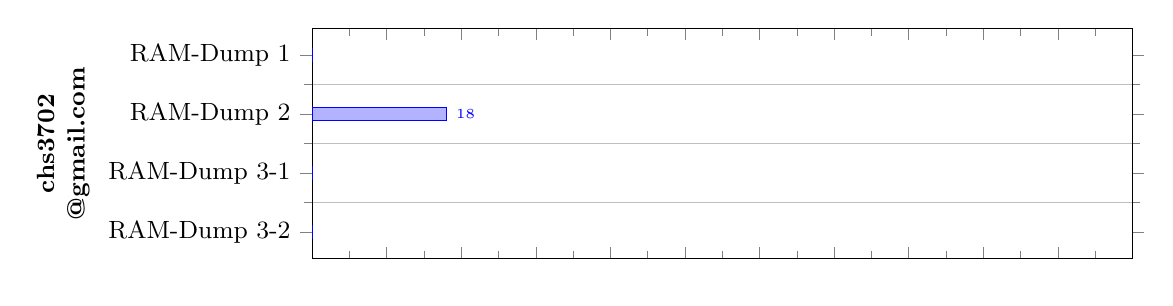
\begin{tikzpicture}
			\begin{axis}[
			xbar,
			width=12cm, 
			height=3cm, 
			ylabel style={align=center}, ylabel=\textbf{chs3702}\\\textbf{@gmail.com},
			y=0.75cm,
			symbolic y coords={RAM-Dump 3-2, RAM-Dump 3-1, RAM-Dump 2, RAM-Dump 1},
			label style={font=\small},
			tick label style={font=\small},
			ytick=data,
			xticklabels={,,},
            xmin = 0,
            xmax = 110,
			nodes near coords, 
			nodes near coords align={horizontal},
			nodes near coords style={font=\tiny},
   			nodes near coords={\pgfmathfloatifflags{\pgfplotspointmeta}{0}{}{\pgfmathprintnumber{\pgfplotspointmeta}}},
			bar width=.17cm,
			enlarge y limits={abs=2*\pgfplotbarwidth},
			scaled x ticks=false,
			legend style={
				at={(0.5,-0.1)},
				anchor=north
			},
			legend columns=3,
    		yminorgrids = true,minor tick num=1
			]
				\addplot coordinates {
				(0,RAM-Dump 3-2)  (0,RAM-Dump 3-1) (18,RAM-Dump 2) (0,RAM-Dump 1)
				};
%				\addplot coordinates {
%				(0,RAM-Dump 3-2)  (0,RAM-Dump 3-1) (0,RAM-Dump 2) (0,RAM-Dump 1)
%				};
%				\addplot coordinates {
%				(0,RAM-Dump 3-2)  (0,RAM-Dump 3-1) (0,RAM-Dump 2) (0,RAM-Dump 1)
%				};
%				\legend{firefox.exe, tor.exe, Andere Prozesse}
			\end{axis}
		\end{tikzpicture}
		\\[-7pt]
		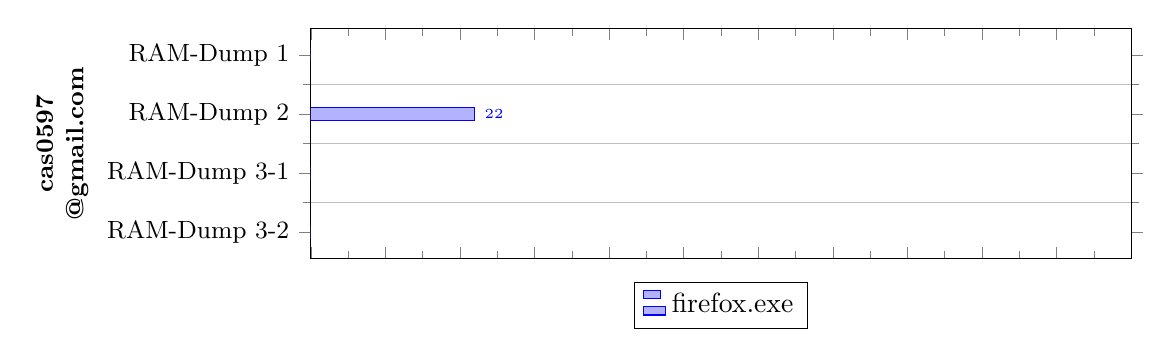
\begin{tikzpicture}
			\begin{axis}[
			xbar,
			width=12cm, 
			height=3cm, 
			ylabel style={align=center}, ylabel=\textbf{cas0597}\\\textbf{@gmail.com},
			y=0.75cm,
			symbolic y coords={RAM-Dump 3-2, RAM-Dump 3-1, RAM-Dump 2, RAM-Dump 1},
			label style={font=\small},
			tick label style={font=\small},
			ytick=data,
			xticklabels={,,},
            xmin = 0,
            xmax = 110,
			nodes near coords, 
			nodes near coords align={horizontal},
			nodes near coords style={font=\tiny},
   			nodes near coords={\pgfmathfloatifflags{\pgfplotspointmeta}{0}{}{\pgfmathprintnumber{\pgfplotspointmeta}}},
			bar width=.17cm,
			enlarge y limits={abs=2*\pgfplotbarwidth},
			scaled x ticks=false,
			legend style={
				at={(0.5,-0.1)},
				anchor=north
			},
			legend columns=3,
    		yminorgrids = true,minor tick num=1
			]
				\addplot coordinates {
				(0,RAM-Dump 3-2)  (0,RAM-Dump 3-1) (22,RAM-Dump 2) (0,RAM-Dump 1)
				};
%				\addplot coordinates {
%				(0,RAM-Dump 3-2)  (0,RAM-Dump 3-1) (0,RAM-Dump 2) (0,RAM-Dump 1)
%				};
%				\addplot coordinates {
%				(0,RAM-Dump 3-2)  (0,RAM-Dump 3-1) (0,RAM-Dump 2) (0,RAM-Dump 1)
%				};
				\legend{firefox.exe}
			\end{axis}
		\end{tikzpicture}
	\end{tabular}
	}
	\captionof{figure}{Gefundene E-Mail Artefakte im Tor RAM}
	\label{chart:tor-volatility-mail}
\end{table}
%\begin{figure}[h!]
%	\centerline{\resizebox{\linewidth}{!}{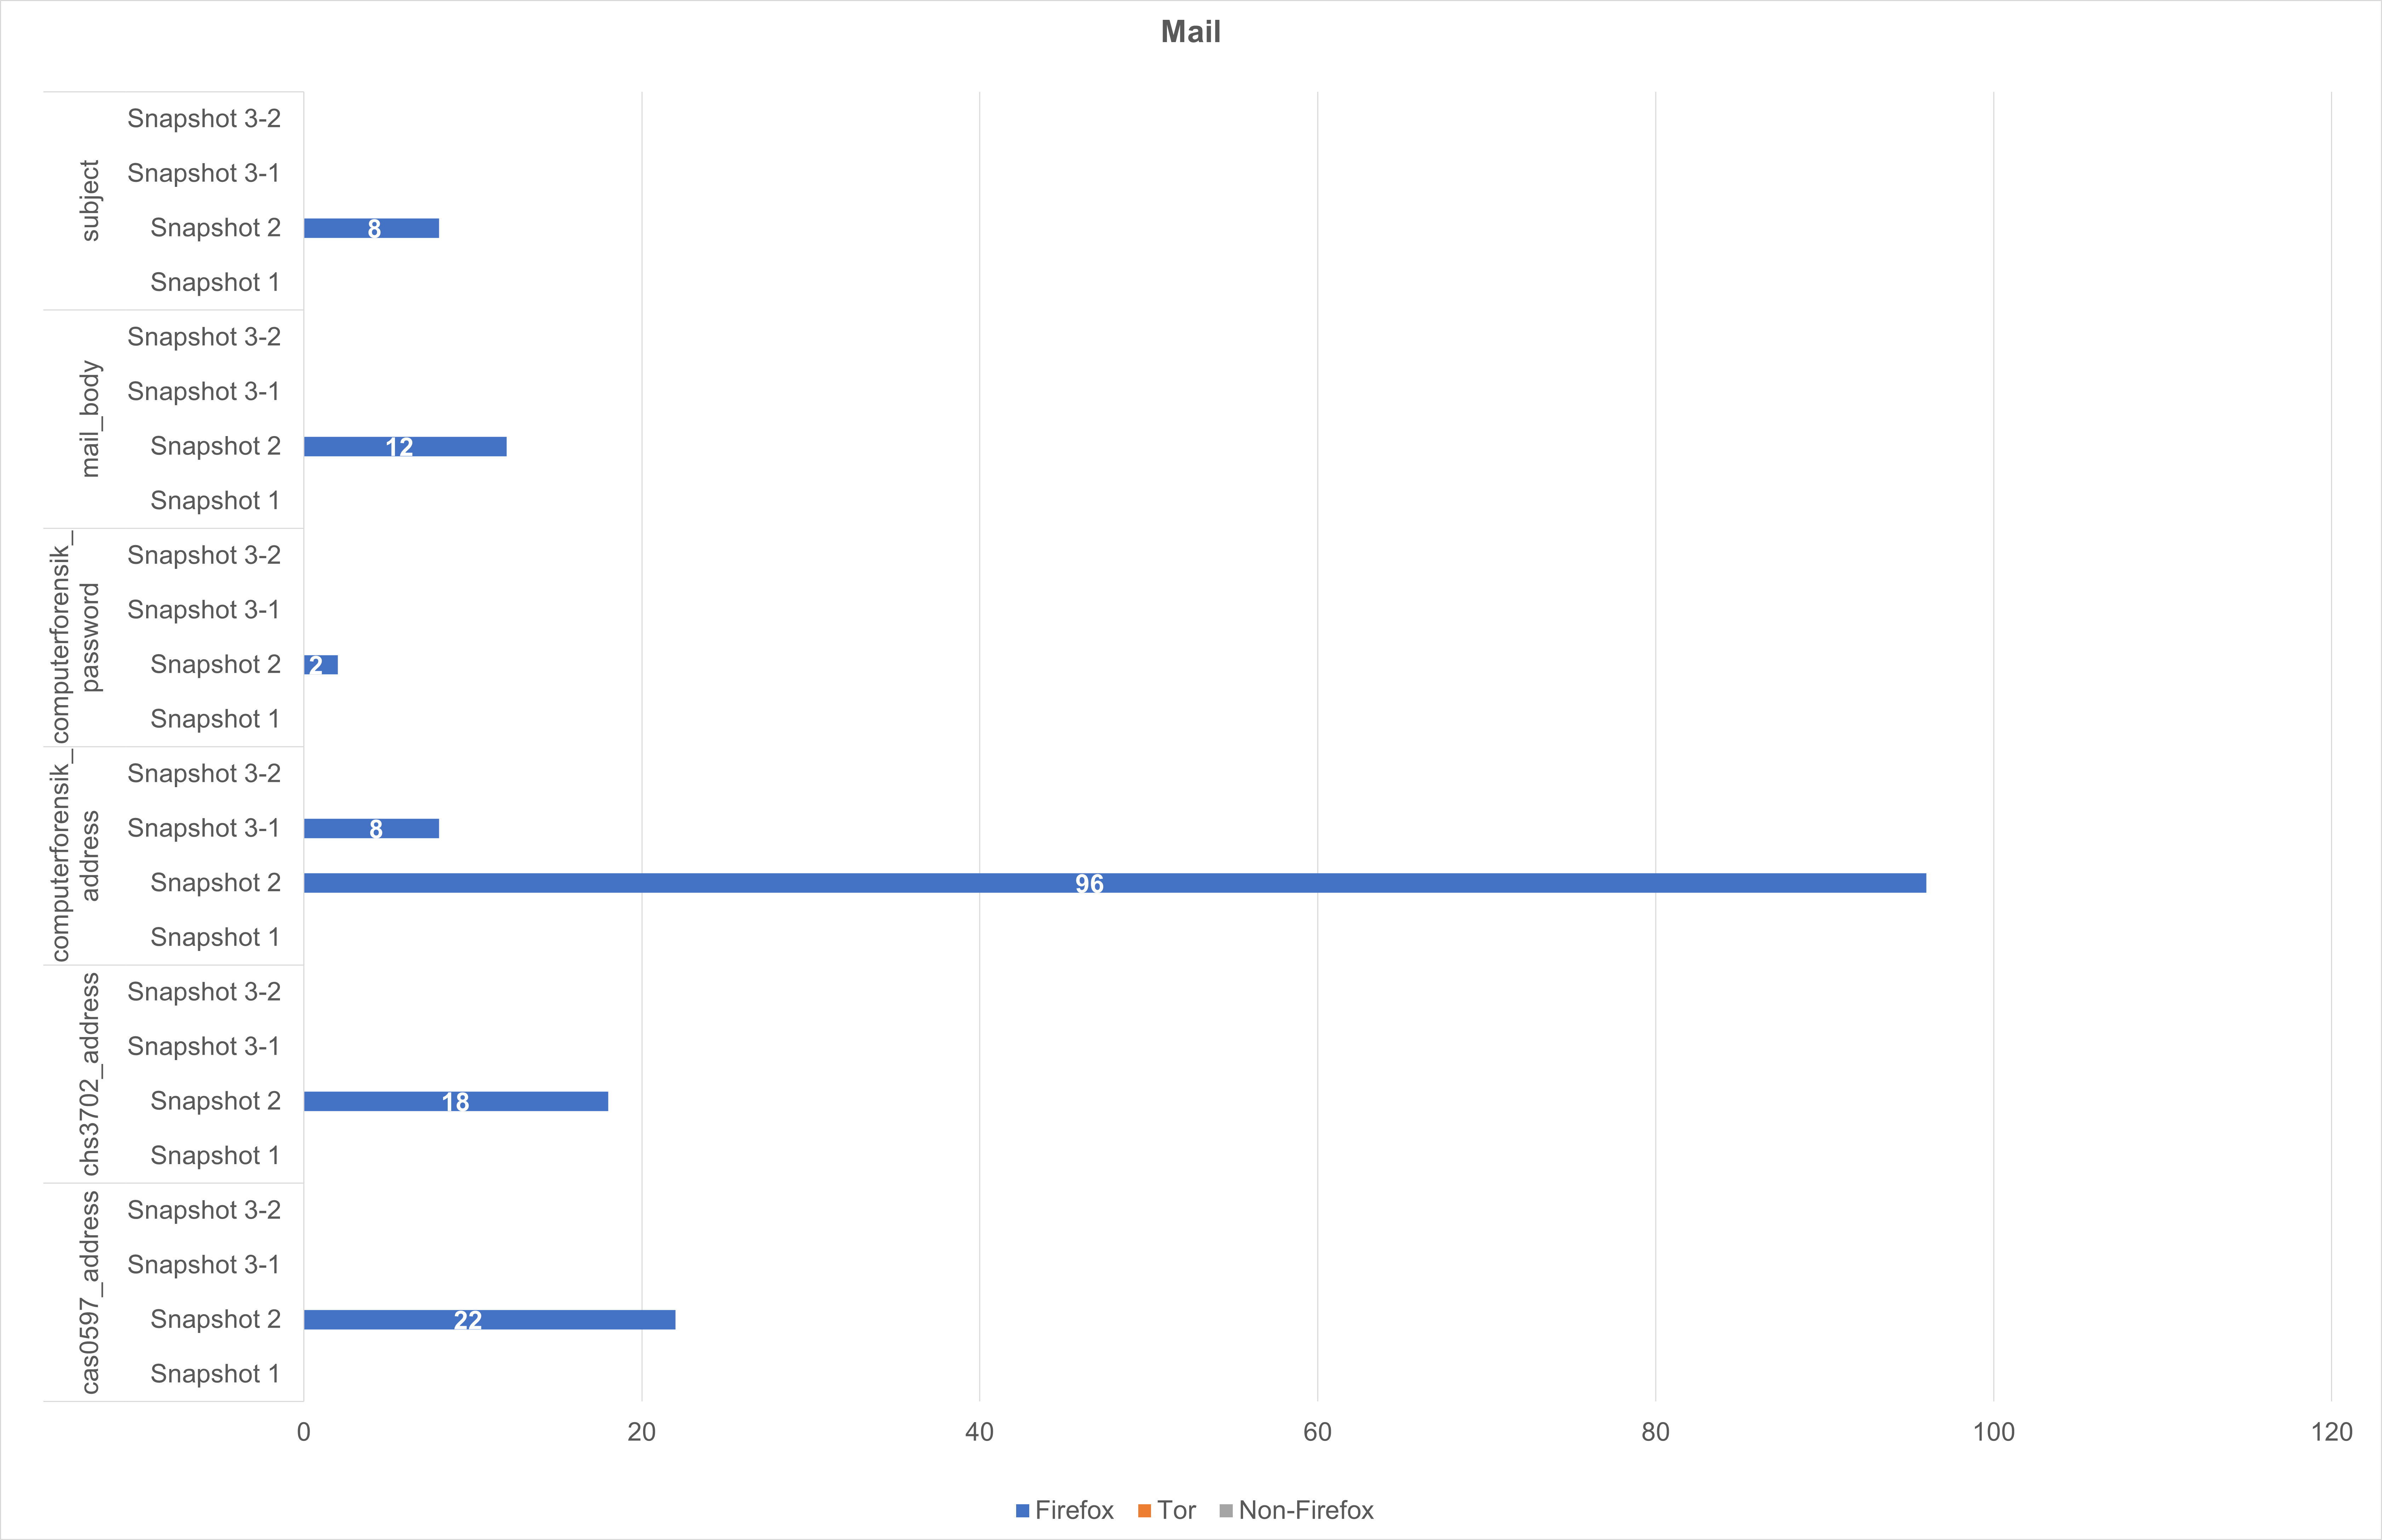
\includegraphics{bilder/volatility/tor/mail.png}}}
%	\label{chart:final-criteria}  
%	\caption{Mail}
%\end{figure}
Wie in Abbildung \ref{chart:tor-volatility-mail} zu sehen ist, wurden die Artefakte ausschließlich in Firefox Prozess gefunden.
Nur die Absenderadresse ``computerforensikvl@gmail.com`` wurde nach Erstellen der neuen Identität in RAM-Dump 3-1 gefunden. Die Absenderadresse ist ebenso das am häufigsten gefundene E-Mail Artefakt.
Wie bei Firefox in Kapitel \ref{subsubsection:ergebnisse-firefox-uncommonlocations-analysemitvolatility} wurde das Passwort als Klartext nach dem Browsing-Szenario im zweiten RAM-Dump gefunden.
Das Passwort wurde in zwei Mal im Firefox Prozess mit der PID 708 gefunden. Tabelle \ref{tab:tor-mapping-virtaddr-to-byteoffset} zeigt die virtuellen Speicheradressen der Artefakte aus der Yarascan Ausgabe sowie deren Abbildung auf die mithilf des Volatility Plugins \textit{memmap} identifizierten Byte-Offsets der extrahierten Speicherseiten.
\begin{table}[h!]
	\resizebox{\linewidth}{!}{
	\begin{tabular}{|c|c|c|ll}
	\cline{1-3}
	\textbf{Virtuelle Speicheradresse} & \textbf{PID} & \textbf{Byte-Offset in extrahierter Speicherseite} &  &  \\ \cline{1-3}
	0x2b1e2c22318                      & 708         & 0xea0318                                         &  &  \\ \cline{1-3}
	0x2b1e2ecb748                     & 708         & 0x10f7748                                         &  &  \\ \cline{1-3}
	\end{tabular}
	}
	\caption{Abbildung der virtellen Speicheradressen der gefundenen Strings im Tor-RAM auf Byte-Offsets der entsprechenden Speicherseiten}
	\label{tab:tor-mapping-virtaddr-to-byteoffset}
\end{table}


\begin{figure}[h!]
	\centering
	\subcaptionbox{Byte-Offset 0xea0318}{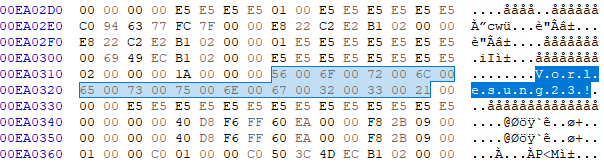
\includegraphics[width=0.47\textwidth]{bilder/volatility/tor/password_0xea0318.png}}%
	\hfill
	\subcaptionbox{Byte-Offset 0x10f7748}{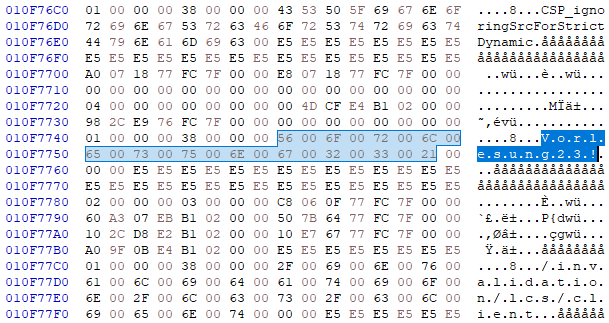
\includegraphics[width=0.47\textwidth]{bilder/volatility/tor/password_0x10f7748.png}}%
	\caption{Passwort-Klartext in Firefox Speicherseiten von PID 708}
	\label{img:firefox-pw-offset-pid-708}  
\end{figure}
Bei Untersuchung des String-Kontexts wurden für das Passwort am Byte-Offset \texttt{0xea0318} wie in Abbildung \ref{img:firefox-pw-offset-pid-708} gezeigt keine Auffällige Artefakte entdeckt.
Im Bereich des gefundenen Passworts am Byte-Offset \texttt{0x10f7748} der String ``CSP\_ignoringSrcForStrictDynamic``, dessen Bedeutung nicht bestimmt werden konnte.
Weiterhin wurde die Zeichenkette ``invalidation/lcs/client`` in der Nähe des Passworts gefunden. Dieser String wird in einem Firefox Bug-Ticket verwendet, welches vor 2017 geschlossen wurde. Der Bug betraf ein Speicher-Leck. \cite{Bugzilla.05.06.2023}
	
\paragraph*{Yara-Regel ``DK-Logo``}
Wie in Abbildung \ref{chart:tor-volatility-image} dargestellt, wurde der Hexadezimal-Wert des Donaukurier-Logos  ein einziges Mal nach dem Browsing Szenario, vor Erstellen der ``Neuen Identität`` im zweiten RAM-Dump in einem Firefox Prozess gefunden.
\begin{figure}[h!]
	\resizebox{\linewidth}{!}{
		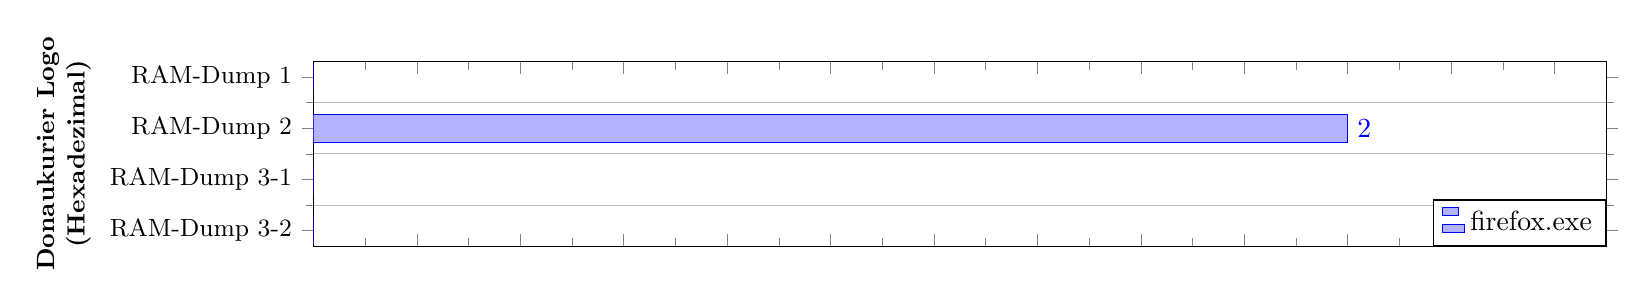
\begin{tikzpicture}
			\begin{axis}[
			xbar,
			width=18cm, 
			height=12cm, 
			ylabel style={align=center}, ylabel=\textbf{Donaukurier Logo}\\\textbf{(Hexadezimal)},
			y=0.65cm,
			symbolic y coords={RAM-Dump 3-2, RAM-Dump 3-1, RAM-Dump 2, RAM-Dump 1},
			label style={font=\small},
			tick label style={font=\small},
			ytick=data,
			xticklabels={,,},
            xmin = 0,
            xmax = 2.5,
			nodes near coords, 
			nodes near coords align={horizontal},
   			nodes near coords={\pgfmathfloatifflags{\pgfplotspointmeta}{0}{}{\pgfmathprintnumber{\pgfplotspointmeta}}},	
			legend style={
				at={(1,0)},
				anchor=south east
			},
			legend columns=2,
    		yminorgrids = true,minor tick num=1
			]
				\addplot coordinates {
				(0,RAM-Dump 3-2)  (0,RAM-Dump 3-1) (2,RAM-Dump 2) (0,RAM-Dump 1)
				};
				\legend{firefox.exe}
			\end{axis}
		\end{tikzpicture}
	}
	\caption{Gefundener Hexadezimalwert des Donaukurier-Logos im Tor RAM}
	\label{chart:tor-volatility-image}
\end{figure}
%\begin{figure}[h!]
%	\centerline{\resizebox{\linewidth}{!}{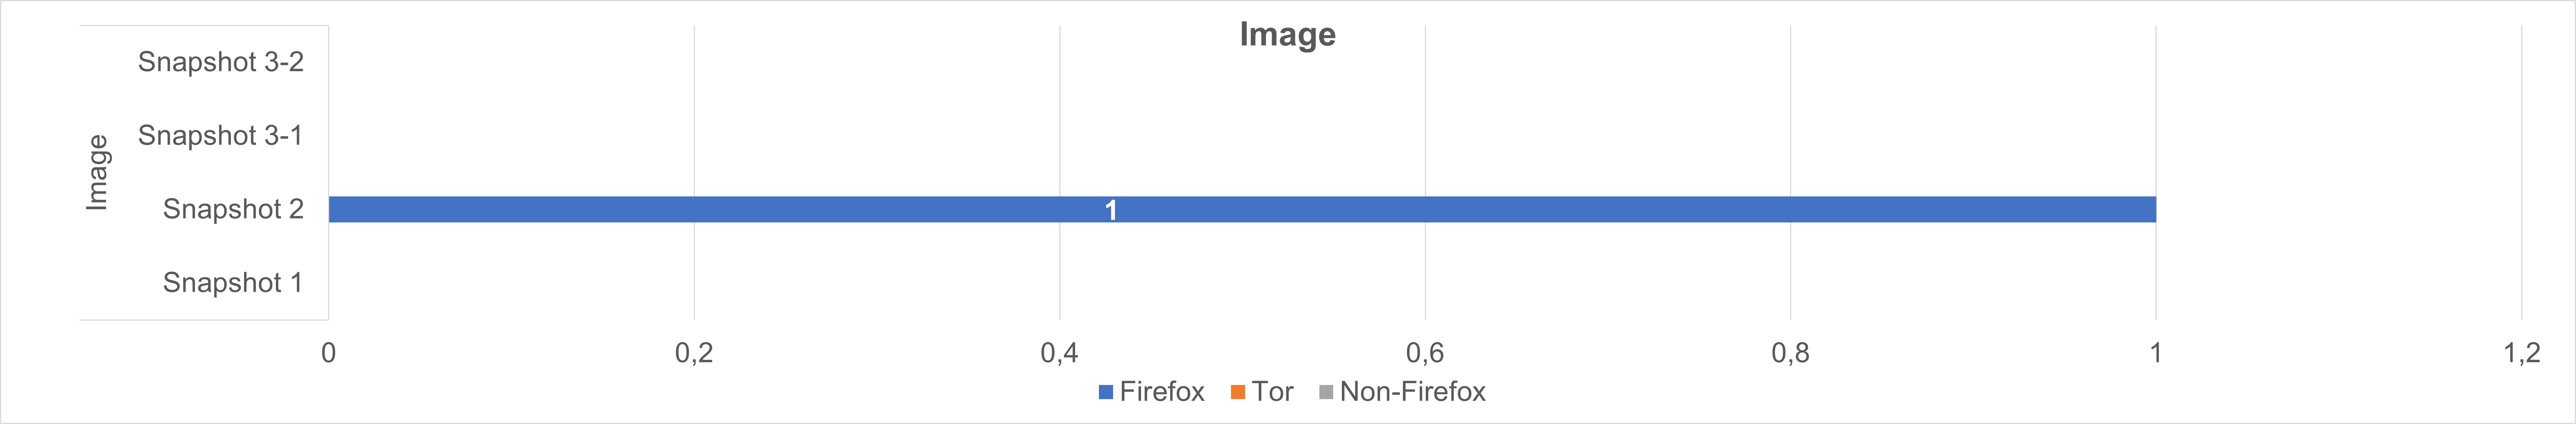
\includegraphics{bilder/volatility/tor/image.png}}}
%	\label{chart:final-criteria}  
%	\caption{Image}
%\end{figure}


%\begin{figure}[h!]
%	\centerline{\resizebox{\linewidth}{!}{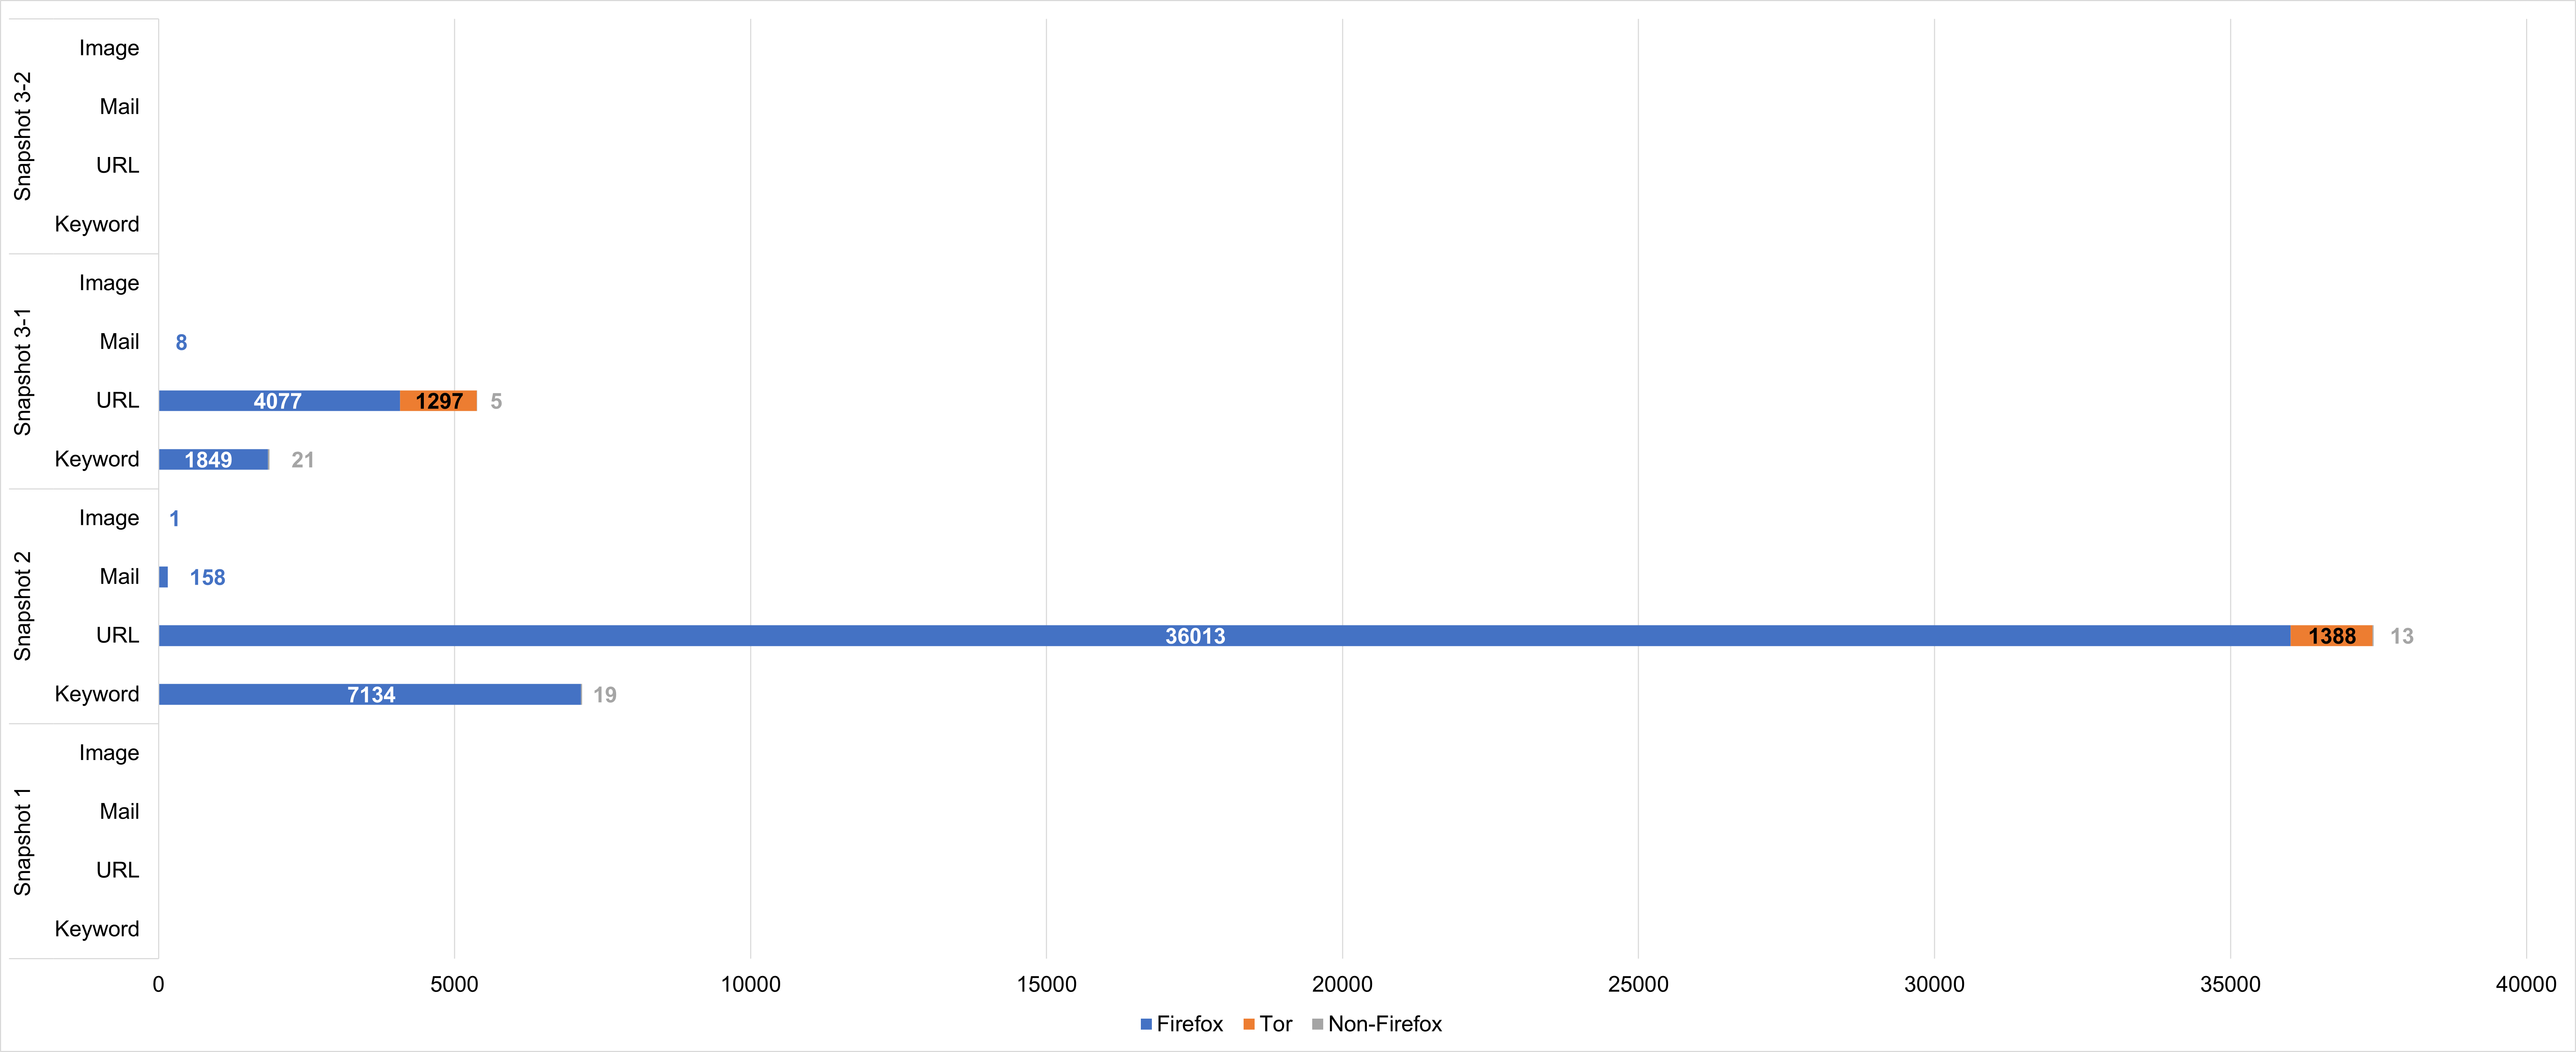
\includegraphics{bilder/volatility/tor/summary.png}}}
%	\label{chart:final-criteria}  
%	\caption{Summary}
%\end{figure}
%Literatur:
%o Autopsy: \cite{Muir.2019}
%	•	Configuration files, downloaded files, and browserrelated data are recoverable from the file system.
%	•	Significant data-leakage from the browsing session occurred: HTTP header information, titles of web pages and an instance of a URL were found in registry files, system files, and unallocated space.
%o RAM-Analyse nach \cite{Muir.2019}:
%	•	Live-Analyse identifiziert auch nach dem Schließen und Deinstallieren des Browsers und Abmelden des Benutzers Spuren von Tor-Prozessen, einschließlich des absoluten Pfads zur Browser-Executable, des Benutzernamens und des Geräts, von dem es ausgeführt wurde.
%	•	The data-leakage contained the German word for ’search’ in reference to a Google search. This hints at the locale of the Tor server used to exit the network (exit relay).
%
%o RAM-Analyse nach \cite{Hariharan.2022}:
%	o	process was found to be firefox.exe
%	o	pslist and pstree: parent process was shown 
%	o	Belkasoft Ram Capturer: retrieve information about facebook
%	o	Cmdline: file path of the browser “E:/TorBrowser/Browser/firefox.exe” + name of process tor.exe and firefox.exe
%	o	Dlllist: DLL files of the executable files were not captured
%	o	Netscan: tor.exe + obfs4proxy.exe -> showed “LISTENING” connections to nonstandardized ports as output.
%	Yarascan: was able to retrieve all the browsing sessions
%o RAM-Analyse nach \cite{Sajan.2021} mit Volatility
%	•	process list extracted from the memory
%	•	registry hives been extracted from the memory dump
%	•	threads were extracted: “D:/VolatilityWorkbench/volatility.exe”–plugins=”D:/VolatilityWorkbench/profiles” pslistfilename =”C:/Users/username/Desktop/tor.raw” –profile=Win10x64 17763 –kdbg=0xf807606ac5e0
%	•	Handles: resources used by the process 5672
%	•	Dlls: These dlls can be found from prefetch file --> Can be found in “prefetch” file -> Analyzed with “winprefetchview”
%	•	Places.sqlite: SQLite viewer has been used to recover bookmarks and frequently visited sites even after uninstalling the application
%	•	Visited Websites: Using keyword search in Dump’s Hex
%
%o Registry:
%	> Shellactivites (siehe Firefox) \cite{Muir.2019}: instance of a URL were found in registry file
%	> \cite{Nelson.2020} The userassist key is located in the NTUSER.dat hive of the
%		 -> Registry and indicates the execution path of the program, as well as the number of times the program was executed 

\subsection*{Registry}
Wie in der Methodik in Kapitel \ref{subsection:methodik-datenanalyse-registry} beschrieben, teilt sich die Analyse der Registry sowohl Common als auch Uncommon Locations. Weder in den Process Monitor ``SetValue`` Operations noch über die Stringsuche in den System- und User-Hives konnten PB Artefakte gefunden werden. Eine detaillierte Analyse der Registry ist im Anhang \ref{subsection:appendix-firefox-registry} beschrieben. 

\section{Chrome}

\subsection*{Uncommon Locations}

o Autopsy Keyword-Suche: 
	> Chrome and Edge produced five artefacts as reported by both tools. (FTK, Autopsy) \cite{Gabet.2018}
		--> Artefakte werden nicht genannt!
	> only two temporary files (Figure 7) were recovered with Minitool Power Data Recovery but it was a dead end; Location: appdata/…/Chrome/…/ Preferences/RF1533fa.TMP \cite{Fayyad.2021}
	> pagefile.sys file showed no traces at all \cite{Said.2011}
	

\section{Brave}